\documentclass[12pt,a4paper]{article}

% --- Language and encoding ---
\usepackage[T2A]{fontenc}
\usepackage[utf8]{inputenc}
\usepackage[russian,english]{babel}

% --- Page geometry ---
\usepackage[a4paper,top=2.5cm,bottom=2.5cm,left=3cm,right=2cm]{geometry}
\usepackage{setspace}
\onehalfspacing

% --- Math, tables, graphics ---
\usepackage{amsmath,amssymb}
\usepackage{booktabs}
\usepackage{graphicx}
\usepackage{adjustbox}
\usepackage{array}
\usepackage{caption}
\usepackage{subcaption}
\usepackage{hyperref}
\hypersetup{hidelinks}
\usepackage{title_page}
\usepackage{enumitem}
\usepackage[protrusion=true,expansion=false]{microtype}
\usepackage[subsection,below]{placeins}  % \FloatBarrier at every \subsection
% Allow slightly looser spacing to avoid Overfull hbox warnings
\sloppy
\emergencystretch=3em

% --- Auto-generated dynamic values ---
% Auto-generated by scripts/generate_values.py. DO NOT EDIT.
% Source: /home/kifbell/sweets/twix/agents_workdir/voice-bench-stats.json

\newcommand{\valNRowsAnalysed}{6680}
\newcommand{\valNProviders}{11}
\newcommand{\valNSpeakers}{20}
\newcommand{\valNUtterancesPerSpeaker}{20}
\newcommand{\valHOneTtsFrontierSize}{6}
\newcommand{\valHOneTtsFrontierTotal}{9}
\newcommand{\valHOneTtsFrontierMembers}{Azure Neural, CosyVoice2, F5-TTS, Google Neural2, OpenAI tts-1, XTTSv2}
\newcommand{\valHOneTtsVerdict}{\textbf{подтверждена}}
\newcommand{\valHOneCloningFrontierSize}{7}
\newcommand{\valHOneCloningFrontierTotal}{8}
\newcommand{\valHOneCloningFrontierMembers}{CosyVoice2, ElevenLabs, F5-TTS, Fish-Speech~S1, Fish-Speech~S2~Pro, Resemble, Typecast}
\newcommand{\valHOneCloningVerdict}{\textbf{подтверждена}}
\newcommand{\valHTwoTtsNatRho}{0.500}
\newcommand{\valHTwoTtsNatPval}{0.170}
\newcommand{\valHTwoTtsNatN}{9}
\newcommand{\valHTwoTtsNatVerdict}{\textbf{не подтверждена}}
\newcommand{\valHTwoCloningNatRho}{-0.190}
\newcommand{\valHTwoCloningNatPval}{0.651}
\newcommand{\valHTwoCloningNatN}{8}
\newcommand{\valHTwoCloningNatVerdict}{\textbf{не подтверждена}}
\newcommand{\valHTwoCloningSimRho}{0.976}
\newcommand{\valHTwoCloningSimPval}{$< 0.001$}
\newcommand{\valHTwoCloningSimN}{8}
\newcommand{\valHTwoCloningSimVerdict}{\textbf{не подтверждена}}
% H3 TOST equivalence test values.
\newcommand{\valHThreeTtsUtmosDelta}{0.200}
\newcommand{\valHThreeTtsUtmosMeanCommercial}{3.734}
\newcommand{\valHThreeTtsUtmosMeanOpenSource}{3.580}
\newcommand{\valHThreeTtsUtmosMeanDiff}{$+0.154$}
\newcommand{\valHThreeTtsUtmosPval}{0.338}
\newcommand{\valHThreeTtsUtmosVerdict}{\textbf{не подтверждена}}
\newcommand{\valHThreeTtsNisqaMosDelta}{0.200}
\newcommand{\valHThreeTtsNisqaMosMeanCommercial}{4.928}
\newcommand{\valHThreeTtsNisqaMosMeanOpenSource}{4.553}
\newcommand{\valHThreeTtsNisqaMosMeanDiff}{$+0.374$}
\newcommand{\valHThreeTtsNisqaMosPval}{0.849}
\newcommand{\valHThreeTtsNisqaMosVerdict}{\textbf{не подтверждена}}
\newcommand{\valHThreeTtsWhisperWerDelta}{0.050}
\newcommand{\valHThreeTtsWhisperWerMeanCommercial}{0.037}
\newcommand{\valHThreeTtsWhisperWerMeanOpenSource}{0.040}
\newcommand{\valHThreeTtsWhisperWerMeanDiff}{$-0.003$}
\newcommand{\valHThreeTtsWhisperWerPval}{$< 0.001$}
\newcommand{\valHThreeTtsWhisperWerVerdict}{\textbf{подтверждена}}
\newcommand{\valHThreeCloningUtmosDelta}{0.200}
\newcommand{\valHThreeCloningUtmosMeanCommercial}{3.436}
\newcommand{\valHThreeCloningUtmosMeanOpenSource}{3.401}
\newcommand{\valHThreeCloningUtmosMeanDiff}{$+0.035$}
\newcommand{\valHThreeCloningUtmosPval}{0.184}
\newcommand{\valHThreeCloningUtmosVerdict}{\textbf{не подтверждена}}
\newcommand{\valHThreeCloningNisqaMosDelta}{0.200}
\newcommand{\valHThreeCloningNisqaMosMeanCommercial}{4.817}
\newcommand{\valHThreeCloningNisqaMosMeanOpenSource}{4.705}
\newcommand{\valHThreeCloningNisqaMosMeanDiff}{$+0.113$}
\newcommand{\valHThreeCloningNisqaMosPval}{0.160}
\newcommand{\valHThreeCloningNisqaMosVerdict}{\textbf{не подтверждена}}
\newcommand{\valHThreeCloningWhisperWerDelta}{0.050}
\newcommand{\valHThreeCloningWhisperWerMeanCommercial}{0.035}
\newcommand{\valHThreeCloningWhisperWerMeanOpenSource}{0.041}
\newcommand{\valHThreeCloningWhisperWerMeanDiff}{$-0.006$}
\newcommand{\valHThreeCloningWhisperWerPval}{$< 0.001$}
\newcommand{\valHThreeCloningWhisperWerVerdict}{\textbf{подтверждена}}
\newcommand{\valHThreeCloningWavlmSimDelta}{0.050}
\newcommand{\valHThreeCloningWavlmSimMeanCommercial}{0.942}
\newcommand{\valHThreeCloningWavlmSimMeanOpenSource}{0.957}
\newcommand{\valHThreeCloningWavlmSimMeanDiff}{$-0.015$}
\newcommand{\valHThreeCloningWavlmSimPval}{0.001}
\newcommand{\valHThreeCloningWavlmSimVerdict}{\textbf{подтверждена}}
\newcommand{\valHThreeCloningEcapaSimDelta}{0.050}
\newcommand{\valHThreeCloningEcapaSimMeanCommercial}{0.665}
\newcommand{\valHThreeCloningEcapaSimMeanOpenSource}{0.732}
\newcommand{\valHThreeCloningEcapaSimMeanDiff}{$-0.067$}
\newcommand{\valHThreeCloningEcapaSimPval}{0.664}
\newcommand{\valHThreeCloningEcapaSimVerdict}{\textbf{не подтверждена}}
\newcommand{\valCalibWavlmUpperPFifty}{0.958}
\newcommand{\valCalibWavlmLowerMean}{0.686}
\newcommand{\valCalibWavlmUpperN}{100}
\newcommand{\valCalibWavlmLowerN}{190}
\newcommand{\valCalibEcapaUpperPFifty}{0.703}
\newcommand{\valCalibEcapaLowerMean}{0.223}
\newcommand{\valCalibEcapaUpperN}{100}
\newcommand{\valCalibEcapaLowerN}{190}
\newcommand{\valBestTtsUtmosProvider}{cosyvoice2}
\newcommand{\valBestTtsUtmosValue}{3.950}
\newcommand{\valWorstTtsUtmosProvider}{fish\_speech\_s1}
\newcommand{\valWorstTtsUtmosValue}{3.403}
\newcommand{\valBestTtsNisqaMosProvider}{google\_tts}
\newcommand{\valBestTtsNisqaMosValue}{5.012}
\newcommand{\valWorstTtsNisqaMosProvider}{fish\_speech\_s1}
\newcommand{\valWorstTtsNisqaMosValue}{4.042}
\newcommand{\valBestTtsWhisperWerProvider}{google\_tts}
\newcommand{\valBestTtsWhisperWerValue}{0.036}
\newcommand{\valWorstTtsWhisperWerProvider}{fish\_speech\_s1}
\newcommand{\valWorstTtsWhisperWerValue}{0.044}
\newcommand{\valBestTtsCostUsdProvider}{cosyvoice2}
\newcommand{\valBestTtsCostUsdValue}{0.0000}
\newcommand{\valWorstTtsCostUsdProvider}{elevenlabs}
\newcommand{\valWorstTtsCostUsdValue}{0.0035}
\newcommand{\valBestTtsLatencySecondsProvider}{google\_tts}
\newcommand{\valBestTtsLatencySecondsValue}{0.302}
\newcommand{\valWorstTtsLatencySecondsProvider}{fish\_speech\_s2\_pro}
\newcommand{\valWorstTtsLatencySecondsValue}{37.030}
\newcommand{\valBestCloningUtmosProvider}{cosyvoice2}
\newcommand{\valBestCloningUtmosValue}{3.666}
\newcommand{\valWorstCloningUtmosProvider}{typecast}
\newcommand{\valWorstCloningUtmosValue}{3.184}
\newcommand{\valBestCloningNisqaMosProvider}{resemble}
\newcommand{\valBestCloningNisqaMosValue}{4.912}
\newcommand{\valWorstCloningNisqaMosProvider}{xtts\_v2}
\newcommand{\valWorstCloningNisqaMosValue}{4.486}
\newcommand{\valBestCloningWhisperWerProvider}{typecast}
\newcommand{\valBestCloningWhisperWerValue}{0.034}
\newcommand{\valWorstCloningWhisperWerProvider}{f5\_tts}
\newcommand{\valWorstCloningWhisperWerValue}{0.043}
\newcommand{\valBestCloningWavlmSimProvider}{cosyvoice2}
\newcommand{\valBestCloningWavlmSimValue}{0.964}
\newcommand{\valWorstCloningWavlmSimProvider}{resemble}
\newcommand{\valWorstCloningWavlmSimValue}{0.937}
\newcommand{\valBestCloningEcapaSimProvider}{cosyvoice2}
\newcommand{\valBestCloningEcapaSimValue}{0.788}
\newcommand{\valWorstCloningEcapaSimProvider}{resemble}
\newcommand{\valWorstCloningEcapaSimValue}{0.630}
\newcommand{\valBestCloningCostUsdProvider}{cosyvoice2}
\newcommand{\valBestCloningCostUsdValue}{0.0000}
\newcommand{\valWorstCloningCostUsdProvider}{typecast}
\newcommand{\valWorstCloningCostUsdValue}{0.0156}
\newcommand{\valBestCloningLatencySecondsProvider}{elevenlabs}
\newcommand{\valBestCloningLatencySecondsValue}{1.131}
\newcommand{\valWorstCloningLatencySecondsProvider}{fish\_speech\_s2\_pro}
\newcommand{\valWorstCloningLatencySecondsValue}{36.177}


% --- Figure path ---
\graphicspath{{figures/}}

\begin{document}

\setTitle{Сравнительный бенчмарк коммерческих и open-source систем синтеза речи и клонирования голоса на основе автоматических метрик качества}
\setStudent{Беляков Кирилл}
\setGroup{ЭАД2026}
\setStudentDate{\today}
\setAdvisor{Dzyabura Daria}
\setAdvisorTitle{Deputy Vice-Rector for Academic Affairs, Full Professor, Academic Director ``Masters in Economic and Data Science''}
\setAdvisorAffiliation{РЭШ}
\setAdvisorDate{2026}
\setYear{2026}
\makeTitlePage

\thispagestyle{empty}
\begin{abstract}
\noindent
Системы синтеза речи и клонирования голоса позволяют генерировать речь по тексту и воспроизводить голос диктора по короткому образцу записи. В настоящее время доступны как коммерческие сервисы, так и модели с открытыми весами, однако их сравнение часто ограничивается отдельными аспектами качества и редко учитывает стоимость и скорость генерации.
В данной работе проводится стандартизированное сравнение \valNProviders{} современных решений, включающее 6 коммерческих сервисов и 5 открытых моделей.
Работа посвящена сравнению современных моделей генерации речи по широкому набору характеристик, выявлению ключевых измерений качества и оценке различий между коммерческими сервисами и моделями с открытыми весами.
Полученные результаты показывают, что ни одна из рассмотренных моделей не является безусловным лидером: в обеих задачах наблюдается широкий Парето-фронт, включающий как коммерческие, так и открытые решения.
Кроме того, различные метрики естественности речи могут приводить к существенно различающимся выводам, тогда как метрики схожести с диктором оказываются практически эквивалентными.
Наконец, сравнение коммерческих сервисов и моделей с открытыми весами не выявляет устойчивого превосходства одной из групп: преимущества зависят от рассматриваемой характеристики.
\end{abstract}
\thispagestyle{empty}
\newpage

\pagenumbering{arabic}
\tableofcontents
\newpage

% =========================================================================
\section{Введение}

\subsection{Контекст и постановка задачи}
Качество синтетической речи приблизилось к человеческому уровню для целого ряда языков и доменов. На рынке одновременно сосуществуют два класса систем: коммерческие облачные сервисы (ElevenLabs, OpenAI TTS, Microsoft Azure Cognitive Services, Google Cloud Text-to-Speech, Typecast, Resemble AI), доступ к которым предоставляется только через платный API, и open-source модели, опубликованные вместе с обученной нейросетью (Coqui XTTSv2, F5-TTS, Alibaba CosyVoice2, FishAudio Fish-Speech S1 и S2 Pro), которые можно запускать на собственной инфраструктуре. При выборе системы для прикладной задачи разработчик сталкивается с тремя методологическими проблемами: (1)~прямая оценка качества речи слушателями плохо воспроизводима между исследованиями и существенно зависит от состава пула слушателей; (2)~существующие публичные сравнения, как правило, измеряют только одну ось качества, не учитывая стоимость и скорость генерации; (3)~опорный набор текстов и дикторов варьируется от исследования к исследованию, что делает прямое сравнение результатов невозможным.

\subsection{Объекты сравнения}
Настоящая работа представляет собой бенчмарк-исследование готовых систем синтеза в режиме инференса; разработка собственных моделей или дообучение существующих весов выходят за рамки работы. Сравнению подлежат \valNProviders{} моделей, которые делятся на две выборки.

Шесть коммерческих облачных API с закрытыми весами: ElevenLabs (модель Multilingual~v2 для TTS, Instant Voice Clone для cloning), OpenAI TTS (\texttt{tts-1}, голос \textit{alloy}), Microsoft Azure Cognitive Services (Neural Voice \texttt{en-US-AvaMultilingualNeural}), Google Cloud Text-to-Speech (\texttt{Neural2-F}, далее --- Google~Neural2), Typecast (модель SSFM-v30, поддерживает только voice cloning) и Resemble AI (Rapid Voice Clone, также cloning-only).

Пять open-source моделей с публично доступными весами; инференс выполнялся на одной видеокарте NVIDIA RTX~4090: Coqui XTTSv2, F5-TTS~\cite{f5tts}, Alibaba CosyVoice2-0.5B~\cite{cosyvoice2}, FishAudio Fish-Speech S1-mini и Fish-Speech S2 Pro.

Все модели запускались с параметрами по умолчанию из документации провайдера, без тюнинга гиперпараметров. Такой подход моделирует поведение типичного разработчика, осуществляющего первичное знакомство с API.

\subsection{Эмпирические данные}
В качестве источника эталонных текстов и опорных записей использован открытый корпус LibriTTS-R~\cite{librittsr} в варианте \textit{test-clean} --- это стандартная для области тестовая подвыборка LibriTTS-R, содержащая чистую студийную читку 39 английских дикторов после шумоподавления исходного LibriTTS моделью DEMUCS. Собственный сбор речевых данных в работе не проводился; корпус является общепризнанным стандартом для сравнения нейронных TTS-моделей (CosyVoice2, XTTSv2, F5-TTS публикуют результаты на нём).

После фильтрации по доступной длительности референса (5--10~секунд) и эталонного аудио целевых утверждений (2--15~секунд) в \textit{test-clean} остаётся 34 пригодных диктора, из которых случайным образом отобраны \valNSpeakers{} с балансом по полу (10 мужчин и 10 женщин); для каждого диктора --- по 20 текстовых утверждений (эмпирический диапазон длины текстов в выборке --- 14--283~символа). Эксперимент покрывает обе задачи синтеза:
\begin{itemize}[noitemsep]
    \item \emph{Text-to-Speech} (фиксированный голос провайдера) --- 9 моделей дают по 400 файлов; Typecast и Resemble не поддерживают TTS-режим.
    \item \emph{Voice cloning} (zero-shot, опорная запись длительностью 5--10~секунд из того же диктора, не входящая в целевые 20 утверждений) --- все 11 моделей; у Resemble AI выборка сокращена до 280 файлов из-за требований к минимальной длине референса.
\end{itemize}
Итоговый объём сгенерированного корпуса --- \valNRowsAnalysed{} файлов.

\subsection{Методология оценки}
В работе применяются исключительно автоматические метрики качества, без привлечения слушателей. Этот выбор продиктован четырьмя аргументами: (i)~воспроизводимость результатов между запусками и независимыми лабораториями, тогда как субъективные MOS-оценки варьируются на 0.2~балла и более между разными пулами слушателей~\cite{voicemos}; (ii)~масштаб эксперимента (\valNRowsAnalysed{}{} файлов), для которого получение хотя бы трёхкратного человеческого MOS требует более 24\,000 субъективных оценок; (iii)~наличие в сообществе устоявшегося прокси --- UTMOSv2~\cite{utmos}, демонстрирующего корреляцию $r \geq 0.94$ с реальным MOS на тест-сплитах VoiceMOS~Challenge~\cite{voicemos}; (iv)~публикация исходных аудиозаписей в открытом доступе позволяет любой третьей стороне применить свои собственные слушательские или автоматические метрики поверх наших данных.

Оценка проводится по пяти метрикам: UTMOSv2 и NISQA~\cite{nisqa} для естественности; Whisper-WER (faster-whisper \textit{medium}, int8 на CPU, с базовой нормализацией текста: нижний регистр, удаление пунктуации, схлопывание пробелов) для разборчивости; WavLM~\cite{wavlm} (с x-vector выходом) и ECAPA-TDNN~\cite{ecapa} для схожести с диктором в задаче voice cloning. Параллельно фиксируются стоимость одной генерации (USD/файл, по официальным прейскурантам провайдеров) и скорость генерации (фактическое время от запроса до получения полного аудиобуфера). Для интерпретации абсолютных значений speaker similarity дополнительно вычислены калибровочные якоря \textit{same-speaker} и \textit{cross-speaker} (Таблица~\ref{tab:calibration}).

% =========================================================================
\section{Обзор литературы}
\label{sec:related-work}

Сравнительные исследования качества систем синтеза речи можно разнести по трём
сложившимся формам. Первая --- открытые лидерборды на основе слушательских
оценок: TTS~Arena~\cite{ttsarena} ранжирует системы по ELO-рейтингу от случайных
слушателей и приводит UTMOSv2 как вторичную метрику; к ограничениям относятся
непрозрачность исходного набора текстов, отсутствие задачи voice cloning, неучёт
стоимости и зависимость рейтинга от ежедневно меняющегося пула. Вторая форма ---
бенчмарки на статичных корпусах в статьях, сопровождающих релизы конкретных
моделей (Seed-TTS~\cite{seedtts}, CosyVoice\,2~\cite{cosyvoice2},
CosyVoice\,3~\cite{cosyvoice3}, XTTS~\cite{xttsv2}, F5-TTS~\cite{f5tts},
VALL-E~\cite{valle} и VALL-E\,2~\cite{valle2}, NaturalSpeech~\cite{naturalspeech} и
NaturalSpeech\,2~\cite{naturalspeech2}); как правило, они сравнивают предлагаемую
модель с открытыми предшественниками на собственной выборке. Третья форма ---
маркетинговые материалы коммерческих провайдеров, где сравнение проводится с
закрытыми данными и закрытым набором метрик, что исключает независимую
верификацию.

Сквозная проблема всех трёх форм --- слабая \emph{воспроизводимость} и почти
полное отсутствие работ, которые одновременно (а)~публикуют не только числа, но и
сами синтезированные аудиозаписи, и (б)~явно сравнивают \emph{ранжирования},
порождаемые разными метриками одного семейства. Именно эти два требования --- ось,
по которой настоящая работа отличается от предшественников. Ниже релевантная
литература рассмотрена по нескольким темам: воспроизводимость оценки и выбор
автоматических метрик; многокритериальные сравнения систем; согласованность метрик
одного семейства и роль выбора эмбеддингов; постановка вопроса о паритете
коммерческих и открытых решений.

% -------------------------------------------------------------------------
\subsection{Воспроизводимость и обоснование автоматических метрик}
\label{ssec:rw-repro}

Прямая оценка слушателями (MOS) считается «золотым стандартом», но плохо
воспроизводима. Chiang, Huang и Lee~\cite{chiang2023} на выборке из 80 статей
INTERSPEECH 2022 показывают, что детали слушательских тестов почти нигде не
сообщаются, и --- что важнее --- на одних и тех же аудио, но при разных настройках
теста получают как минимум три различных ранжирования тех же TTS-моделей. Cooper,
Huang, Toda и Yamagishi~\cite{cooper2022gen} демонстрируют, что автоматические
MOS-предикторы хорошо работают внутри своего теста, но плохо обобщаются на новые
контексты прослушивания, причём невиданные системы --- особенно тяжёлый случай.
Эти две работы --- основное обоснование выбора в пользу исключительно
автоматических, полностью воспроизводимых метрик и публикации самих аудио для
независимой переоценки (ср. позиционную работу об ответственной оценке
TTS~\cite{responsibleeval}). UTMOSv2~\cite{utmos} (наследник UTMOS~\cite{utmosv1},
победитель VoiceMOS~Challenge~\cite{voicemos} в варианте T05~\cite{t05}) и
NISQA~\cite{nisqa,nisqatts} служат стандартными прокси естественности;
% дистрибутивные бенчмарки TTSDS~\cite{ttsds} и TTSDS2~\cite{ttsds2}, а также
% Audio~Turing~Test~\cite{audioturing} и SOMOS~\cite{somos} образуют современный
% методологический контекст.
воспроизводимых же работ, публикующих и метрики, и аудио,
и при этом сравнивающих между собой ранжирования метрик, в литературе крайне мало.

% -------------------------------------------------------------------------
\subsection{Многокритериальные сравнения и отсутствие доминирующей системы}
\label{ssec:rw-multicriteria}

Сравнение систем синтеза одновременно по многим осям --- естественность,
разборчивость, схожесть с диктором, стоимость, скорость --- ставит вопрос о том,
существует ли решение, доминирующее остальные сразу по всем критериям. Большинство
модельно-ориентированных бенчмарков меряют лишь две оси --- WER и speaker
similarity (SIM): протокол Seed-TTS~\cite{seedtts} вычисляет WER через
Whisper~\cite{whisper} и SIM через эмбеддинги WavLM~\cite{wavlm}, и именно этот
протокол де-факто воспроизводят CosyVoice\,2/3~\cite{cosyvoice2,cosyvoice3},
Qwen3-TTS~\cite{qwen3tts} и др. Однако такие сравнения почти никогда не включают
стоимость и скорость как самостоятельные оси. Отдельная работа об отзывчивости
open-source TTS~\cite{berlinski} смещает акцент именно на задержку и пропускную
способность, но не объединяет их с качеством и не охватывает коммерческие API.

Прямых сравнений коммерческих и open-source систем в одном эксперименте мало, и их
выводы неоднородны. EmergentTTS-Eval~\cite{emergenttts} оценивает и проприетарные
(ElevenLabs, Deepgram, OpenAI~4o-mini-tts), и открытые системы через
оценку языковой моделью на сложных просодических примерах и фиксирует разрыв в
пользу закрытых моделей по ряду аспектов. Работа о Human~Fooling~Rate~\cite{hfr}
сравнивает 5~коммерческих и 5~open-source систем на слух 135 участников и приходит
к выводу, что коммерческие модели ближе к «человеческой неотличимости» на
разговорной речи, тогда как open-source отстают. Поскольку эти работы измеряют
разные домены и используют разные метрики, их выводы расходятся --- что показывает,
насколько положение Парето-фронта зависит от выбора осей оценки.
% Аналогичные сравнения «платное
% vs открытое» в соседней задаче ASR (например, бенчмарк PennSound) традиционно
% находят преимущество платных сервисов --- контраст, на фоне которого результат
% становится содержательным, а не ожидаемым.

% -------------------------------------------------------------------------
\subsection{Согласованность автоматических метрик и выбор эмбеддингов}
\label{ssec:rw-metric-agreement}

Метрики одного семейства не обязаны давать одинаковые ранги --- это касается как
метрик естественности (UTMOSv2, NISQA), так и метрик схожести с диктором (WavLM,
ECAPA), и существенно для корректной интерпретации любых сравнений.

\paragraph{Естественность: расхождение и его механизм.} Расхождение между двумя
номинально однотипными метриками естественности не случайно --- в литературе описан
его механизм. Во-первых, MOS-предикторы плохо обобщаются между тестовыми
контекстами и системами~\cite{cooper2022gen}, поэтому две независимо обученные
модели могут давать разный сигнал на новой выборке провайдеров. Во-вторых, для
SOTA-систем объективные метрики страдают \emph{насыщением шкалы}, что делает
ранжирование, особенно по предиктивным MOS-метрикам, ненадёжным: это прямо
показано в работе об итеративном различении (I2D)~\cite{i2d} и согласуется с
наблюдениями TTSDS~\cite{ttsds} о том, что MOS-предикторы лишь иногда коррелируют
с человеческими оценками и в целом не обобщаются. Эти два механизма --- ограниченная
обобщаемость и насыщение --- объясняют, почему две метрики естественности могут
давать расходящиеся системные ранги; NISQA, исторически разработанная для оценки
канала и кодека, дополнительно упирается в верхнюю границу шкалы у провайдеров с
чистым каналом.

\paragraph{Схожесть с диктором: выбор эмбеддингов имеет значение.} Косинусная
близость speaker-эмбеддингов между опорной и синтезированной записью --- основная
объективная метрика клонирования; её валидность как прокси MUSHRA-оценок показана
в~\cite{autospksim}, а на её основе построен открытый бенчмарк клонирования
ClonEval~\cite{cloneval}. При этом результат зависит от того, \emph{какой} энкодер
выбран. Специальное исследование~\cite{embcompare} сравнивает ECAPA-TDNN, x-vector
и H/ASP как энкодеры для оценки speaker similarity в zero-shot multi-speaker TTS и
находит, что выбор энкодера влияет на оценку (ECAPA опережает x-vector, но
оригинальный H/ASP стабильно лучше обоих), подчёркивая необходимость эмпирической
проверки при переиспользовании эмбеддингов из задач распознавания диктора (ср.
применение ECAPA как speaker encoder в multi-speaker TTS~\cite{ecapamultispk}).
Открытым при этом остаётся вопрос, проявляется ли эта чувствительность
преимущественно на уровне отдельных высказываний или сохраняется и на уровне
системных ранжирований. Систематических работ, которые сравнивали бы именно
\emph{ранжирования} двух метрик одного семейства между собой (а не их корреляцию с
человеком), в литературе практически нет.

% -------------------------------------------------------------------------
\subsection{Паритет систем: эквивалентность против тестов на различие}
\label{ssec:rw-equivalence}

Вопрос о том, не уступают ли open-source системы коммерческим, по своей логике
является вопросом об \emph{эквивалентности}, а не о различии, --- и это
методологически нетипично для области синтеза речи. Сложившаяся практика сравнения
TTS ориентирована именно на обнаружение различий: характерна уже работа
Chevelu et al.~\cite{chevelu2015} с подзаголовком «methodology focused on
differences», где отмечается, что случайный выбор сэмплов сглаживает различия и
приводит к ложному выводу о незначимости улучшения. Заявления о «human parity»
также строятся на тестах различия: NaturalSpeech~\cite{naturalspeech} объявляет
паритет с человеком через отсутствие статистически значимой разницы в
Wilcoxon-тесте. Между тем отсутствие значимого различия не равно эквивалентности ---
именно это разграничение лежит в основе процедуры TOST (two one-sided tests), для
которой каноническими методологическими ссылками служат
Lakens~\cite{lakens2017} и Lakens, Scheel и Isager~\cite{lakens2018}: задаётся
наименьший интересующий эффект $\delta$ и проверяются две односторонние гипотезы,
причём авторы прямо предупреждают о распространённой ошибке вывода «эффекта нет» из
статистической незначимости. Применений TOST или non-inferiority-тестирования к
сравнению TTS-систем в литературе обнаружить не удалось.

Сам вопрос о паритете коммерческих и открытых систем в литературе решается
неоднозначно. С одной стороны, разрыв в пользу закрытых систем фиксируют
EmergentTTS-Eval~\cite{emergenttts} на сложных кейсах и работа о
Human~Fooling~Rate~\cite{hfr} на разговорной речи. С другой стороны, независимые
релизы показывают, что на стандартных осях разрыв закрывается:
CosyVoice\,3~\cite{cosyvoice3} заявляет SOTA по content consistency, speaker
similarity и prosody naturalness, а Qwen3-TTS~\cite{qwen3tts} --- наименьший WER на
Seed-TTS и превосходство над коммерческими MiniMax и ElevenLabs по speaker
similarity. Отдельно стоит отметить методологический нюанс: у современных систем
разборчивость упирается в «пол» (WER, близкий к показателям реальной речи;
см.~\cite{ttsds2,i2d}), поэтому эквивалентность сильных систем по WER ожидаема, а
дискриминирующий сигнал смещается с разборчивости на естественность и схожесть с
диктором.

% -------------------------------------------------------------------------
\subsection{Пробел в литературе}
\label{ssec:rw-gap}

Суммируя, в существующей литературе не обнаружено работ, удовлетворяющих
одновременно условиям: (а)~совместное сравнение коммерческих API и open-source
моделей в едином эксперименте на едином корпусе и наборе метрик;
(б)~явный учёт стоимости и скорости генерации как самостоятельных осей;
(в)~публичная доступность как численных результатов, так и самих синтезированных
аудиозаписей для независимой переоценки;
(г)~прямое сравнение \emph{ранжирований}, порождаемых разными метриками одного
семейства (естественность; схожесть с диктором);
(д)~постановка вопроса о паритете двух совокупностей моделей как формального теста
\emph{эквивалентности} (TOST), а не теста на различие.
Настоящая работа закрывает указанный пробел.

% =========================================================================
\section{Цель и вопросы работы}
\label{sec:objective}
\emph{Основной исследовательский вопрос:} \textit{какие из современных систем синтеза речи и клонирования голоса составляют Парето-оптимальное множество в пространстве (естественность, разборчивость, схожесть с диктором, стоимость, скорость генерации) на корпусе LibriTTS-R test-clean (английская студийная речь), и достигли ли open-source модели в среднем эквивалентности с коммерческими моделями по качественным метрикам в пределах методологически значимого порога $\delta$?}

Этот вопрос декомпозируется в три формальные гипотезы, проверяемые в Разделе~\ref{sec:hypotheses}:
\begin{itemize}[noitemsep]
    \item \textbf{H1} (Парето-оптимальность моделей). Не существует модели, парето-доминирующей над всеми остальными в многомерном пространстве оценок: для TTS --- (UTMOSv2, NISQA, Whisper-WER, стоимость); для voice cloning --- (UTMOSv2, NISQA, WavLM-similarity, Whisper-WER, стоимость).
    \item \textbf{H2} (Согласованность метрик). Для естественности (UTMOSv2 vs NISQA) ожидается согласованность системных рангов ($\rho_{\text{Spearman}} \geq 0.7$), поскольку обе метрики номинально измеряют одно и то же свойство. Для speaker similarity (WavLM vs ECAPA) ожидается расхождение ($\rho < 0.7$), поскольку модели имеют разные архитектуры и могут давать разный сигнал. Подтверждение каждой из двух подгипотез означало бы возможность ограничиться одной метрикой в соответствующем семействе.
    \item \textbf{H3} (Эквивалентность коммерческих и open-source моделей). На стандартизованном тесте LibriTTS-R \textit{test-clean} коммерческие модели в среднем не отличаются от open-source моделей по качественным метрикам более чем на методологически значимый порог $\delta$ ни в одну из сторон (двусторонний TOST-тест с $\delta = 0.2$ для UTMOSv2/NISQA, $\delta = 0.05$ для WER и speaker similarity).
\end{itemize}

\medskip
\noindent\emph{Цель работы.} Построить воспроизводимый бенчмарк современных TTS- и voice-cloning-систем на едином корпусе и едином наборе метрик, формализовать сравнительные гипотезы и проверить их статистически. Все артефакты (синтезированные аудиозаписи, метрики, скрипты) выложены публично; повторение эксперимента занимает порядка двух суток на одной видеокарте NVIDIA RTX~4090.

\medskip
\noindent\emph{Вклад работы.}
\begin{itemize}
    \item Собран открытый бенчмарк из \valNRowsAnalysed{} аудиозаписей с фиксированным манифестом текстов и опорных записей.
    \item Реализован унифицированный конвейер обработки, объединяющий пять автоматических метрик качества, а также измерения скорости генерации и стоимости, что устраняет вариативность методологии между провайдерами.
    \item Сформулированы и статистически проверены три гипотезы: о Парето-оптимальности (H1), согласованности метрик (H2) и эквивалентности коммерческих и open-source моделей по качественным метрикам (H3, TOST с практически значимыми порогами $\delta$).
    \item Публично выложены сами синтезированные аудиозаписи (на сетевом хранилище проекта), что позволяет независимым исследователям пересчитать наши метрики или применить альтернативные, в том числе человеческие.
\end{itemize}

% =========================================================================
\section{Автоматические метрики}

\subsection{Корпуса для оценки TTS}
LibriTTS~\cite{libritts} --- стандартный корпус для исследований нейронного TTS, содержащий 585~часов английской речи 2456 дикторов; разделён на чистые и шумные части, сопровождается тщательной нормализацией текстов. LibriTTS-R~\cite{librittsr} --- его улучшенная версия с применённой моделью DEMUCS для шумоподавления. Подвыборка \textit{test-clean} содержит 39~дикторов и широко используется как тестовый сплит в работах по few-shot voice cloning.

\subsection{UTMOSv2 как прокси MOS}
UTMOSv2~\cite{utmos} --- модель предсказания Mean Opinion Score, обученная на корпусах MOS-аннотированных пар (\textit{stimulus, score}) с применением Self-Supervised Learning эмбеддингов WavLM. Достигает корреляции Пирсона $r \geq 0.94$ с реальным MOS на test-сплитах конкурсов VoiceMOS Challenge. В TTS Arena (Hugging Face) UTMOSv2 используется как единая ось ранжирования. Ограничения: значения сжаты в диапазон 3.2--4.0 для современных систем, выдаваемые «как есть» интерпретировать как MOS не следует.

\subsection{NISQA}
NISQA~\cite{nisqa} --- многомерная модель оценки качества телефонной речи, выдаёт пять величин: общее MOS и четыре сабскора (Noisiness, Coloration, Discontinuity, Loudness). Предназначена изначально для оценки кодеков и каналов связи, но активно используется и для TTS. В наших экспериментах наблюдается насыщение шкалы NISQA для коммерческих TTS-провайдеров: значения упираются в верхнюю границу около 5.0.

\subsection{Whisper-WER как метрика разборчивости}
Word Error Rate, или WER, --- стандартная метрика разборчивости синтетической речи, вычисляемая как
\[
\mathrm{WER} \;=\; \frac{S + D + I}{N},
\]
где $S$, $D$, $I$ --- количество замен, удалений и вставок при сравнении ASR-расшифровки с эталонным текстом, $N$ --- общее число слов в эталонной транскрипции. В качестве ASR-системы выбран faster-whisper-\textit{medium} (соответствует выбору в открытом бенчмарке TTSDS, что упрощает сравнение результатов), запущенный в режиме int8 на CPU.

\subsection{Speaker similarity}
Cosine similarity speaker-эмбеддингов между опорной записью диктора и синтезированным аудио --- основная объективная метрика качества voice cloning. Используются две независимые модели:
\begin{itemize}
    \item \emph{WavLM speaker embedding}~\cite{wavlm}: WavLM-Base+, дообученная на VoxCeleb для задачи speaker verification, выход --- x-vector. Калиброванный нами same-speaker $p_{50}$ составляет \valCalibWavlmUpperPFifty{}, cross-speaker mean --- \valCalibWavlmLowerMean{}.
    \item \emph{ECAPA-TDNN}~\cite{ecapa}: классический speaker recognition бэкбон с emphasized channel attention. Same-speaker $p_{50}=\valCalibEcapaUpperPFifty{}$, cross-speaker mean $= \valCalibEcapaLowerMean{}$ --- более широкий динамический диапазон, чем у WavLM.
\end{itemize}
Калибровочные якоря (Таблица~\ref{tab:calibration}) позволяют интерпретировать абсолютные значения схожести.

% Auto-generated. Do not edit.
\begin{table}[ht]
\centering
\caption{Калибровочные якоря для метрик speaker similarity. «Same-speaker» --- cosine similarity между двумя независимыми утверждениями одного диктора (верхняя граница). «Cross-speaker» --- схожесть между разными дикторами (нижняя граница).}
\label{tab:calibration}
\begin{tabular}{lrrrrr}
\toprule
Метрика & Same-speaker $p_{50}$ & Same-speaker mean $\pm$ std & $N_{up}$ & Cross-speaker mean $\pm$ std & $N_{lo}$ \\
\midrule
WAVLM & 0.958 & 0.946 $\pm$ 0.051 & 100 & 0.686 $\pm$ 0.170 & 190 \\
ECAPA & 0.703 & 0.676 $\pm$ 0.153 & 100 & 0.223 $\pm$ 0.118 & 190 \\
\bottomrule
\end{tabular}
\end{table}


% =========================================================================
\section{Методология}
\label{sec:methodology}

\subsection{Дизайн эксперимента}
Эксперимент построен по факториальной схеме «провайдер $\times$ задача $\times$ диктор $\times$ утверждение». Из \textit{test-clean} LibriTTS-R случайно отобраны \valNSpeakers{} дикторов (10 мужчин + 10 женщин), сбалансированных по полу. Для каждого диктора выбраны 20 утверждений с эталонной аудиозаписью длительностью 2--15~секунд, что даёт 400 пар (диктор, текст) на (провайдер, задача); эмпирический диапазон длины текстов в выборке составляет 14--283~символа. Для voice-cloning задачи в качестве reference берётся одна 5--10-секундная запись того же диктора, не входящая в целевые 20 утверждений.

Каждая (провайдер, задача) комбинация даёт ровно 400 аудиозаписей, кроме исключений:
\begin{itemize}
    \item Typecast и Resemble были проверены только на задаче voice cloning (TTS-режим у этих провайдеров отсутствует).
    \item У Resemble 6 дикторов из 20 имеют опорную запись короче 10 секунд, что нарушает требования rapid-clone эндпоинта; они исключены, итого 280 файлов в cloning-задаче.
\end{itemize}
Итоговый объём сгенерированного корпуса --- \valNRowsAnalysed{} файлов; перечень всех строк, попадающих в анализ, приведён в Таблице~\ref{tab:sample_sizes}.

% Auto-generated. Do not edit.
\begin{table}[ht]
\centering
\caption{Размеры выборок: количество файлов с непустым значением каждой метрики, по (провайдер $\times$ задача). Прочерк --- метрика неприменима или не была посчитана.}
\label{tab:sample_sizes}
\resizebox{\textwidth}{!}{%
\begin{tabular}{llrrrrrr}
\toprule
Провайдер & Задача & Файлов & UTMOSv2 & NISQA & WER & WavLM & ECAPA \\
\midrule
Azure Neural & TTS & 400 & 400 & 400 & 400 & 0 & 0 \\
Azure Neural & CLONING & 400 & 400 & 400 & 400 & 0 & 0 \\
CosyVoice2 & TTS & 400 & 400 & 400 & 400 & 0 & 0 \\
CosyVoice2 & CLONING & 400 & 400 & 400 & 400 & 400 & 400 \\
ElevenLabs & TTS & 400 & 400 & 400 & 400 & 0 & 0 \\
ElevenLabs & CLONING & 400 & 400 & 400 & 400 & 400 & 400 \\
F5-TTS & TTS & 400 & 400 & 400 & 400 & 0 & 0 \\
F5-TTS & CLONING & 400 & 400 & 400 & 400 & 400 & 400 \\
Fish-Speech S1 & TTS & 400 & 400 & 400 & 400 & 0 & 0 \\
Fish-Speech S1 & CLONING & 400 & 400 & 400 & 400 & 400 & 400 \\
Fish-Speech S2 Pro & TTS & 400 & 400 & 400 & 400 & 0 & 0 \\
Fish-Speech S2 Pro & CLONING & 400 & 400 & 400 & 400 & 400 & 400 \\
Google Neural2 & TTS & 400 & 400 & 400 & 400 & 0 & 0 \\
Google Neural2 & CLONING & 400 & 400 & 400 & 400 & 0 & 0 \\
OpenAI tts-1 & TTS & 400 & 400 & 400 & 400 & 0 & 0 \\
OpenAI tts-1 & CLONING & 400 & 400 & 400 & 400 & 0 & 0 \\
Resemble & CLONING & 280 & 280 & 280 & 280 & 280 & 280 \\
Typecast & CLONING & 400 & 400 & 400 & 400 & 400 & 400 \\
XTTSv2 & TTS & 400 & 400 & 400 & 400 & 0 & 0 \\
XTTSv2 & CLONING & 400 & 400 & 400 & 400 & 400 & 400 \\
\bottomrule
\end{tabular}%
}
\end{table}


\subsection{Перечень моделей}
Шесть коммерческих API: \textit{ElevenLabs} (Multilingual v2 + IVC clone), \textit{OpenAI TTS} (tts-1, voice = alloy), \textit{Azure Neural Speech} (en-US-AvaMultilingualNeural), \textit{Google~Neural2} (Neural2-F), \textit{Typecast} (SSFM-v30) и \textit{Resemble AI} (rapid clone). Пять open-source моделей: \textit{Coqui XTTSv2}, \textit{F5-TTS}, \textit{Alibaba CosyVoice2-0.5B}, \textit{FishAudio Fish-Speech S1-mini} и \textit{Fish-Speech S2 Pro}. Все open-source модели запускались на одном NVIDIA RTX~4090 (24~ГБ); веса кэшировались на NFS-хранилище между запусками.

\textit{Замечание о cloning-задаче}. Azure~Neural Speech, Google~Neural2 и OpenAI~tts-1 не имеют voice-cloning-эндпоинта: при обращении они синтезируют речь фиксированным голосом провайдера и игнорируют опорную запись диктора. Их строки в cloning-задаче технически генерируются (для возможности расчёта UTMOSv2, NISQA, WER, задержки и стоимости), однако исключаются из всех cloning-аналитик (Парето-фронт, тесты H1 (cloning), H2 (cloning), H3 (cloning)), поскольку структурно эти провайдеры не выполняли оцениваемую задачу. Все вердикты по cloning формируются на 8 моделях: ElevenLabs, Typecast, Resemble, XTTSv2, F5-TTS, CosyVoice2, Fish-Speech~S1, Fish-Speech~S2~Pro.

\subsection{Метрики}
Каждая запись оценивается следующими автоматическими судьями:
\begin{itemize}[noitemsep]
    \item UTMOSv2 --- наследник UTMOS, прокси MOS-оценки естественности.
    \item NISQA-MOS вместе с четырьмя сабскорами (Noisiness, Coloration, Discontinuity, Loudness).
    \item Whisper-WER: faster-whisper \textit{medium} (вариант, использованный также в TTSDS-бенчмарках) в качестве ASR-системы; нормализация ASR-расшифровки и эталонного текста до сравнения --- нижний регистр, удаление пунктуации, схлопывание пробелов.
    \item WavLM speaker embedding с x-vector головой --- косинусная близость эмбеддинга синтезированного аудио и опорной записи диктора, только на cloning-задаче.
    \item ECAPA-TDNN cosine similarity --- аналогично, на основе альтернативного speaker-encoder.
\end{itemize}
Стоимость (USD) рассчитывается по официальным прейскурантам провайдеров (см. Таблицу~\ref{tab:costs}) умножением на число символов исходного текста. Задержка измеряется как фактическое время от вызова сетевого запроса (для облачных API) или метода генерации (для локальных моделей) до получения полного аудиобуфера. Точные версии моделей, идентификаторы весов на Hugging Face и параметры нормализации текста (\texttt{jiwer.Compose}) приведены в репозитории проекта.

\subsection{Калибровка метрик speaker similarity}
Абсолютные значения cosine similarity WavLM и ECAPA не имеют интуитивной шкалы. Для интерпретации мы вычисляем два якоря:
\begin{itemize}[noitemsep]
    \item Верхний (\emph{same-speaker}): схожесть между двумя независимыми записями одного диктора. Усреднение по 100 случайным парам.
    \item Нижний (\emph{cross-speaker}): схожесть между записями разных дикторов. Усреднение по 190 случайным парам.
\end{itemize}
Используя медиану верхнего якоря, можно нормализовать наблюдаемые значения схожести и интерпретировать их как процент достижения «потолка» same-speaker.

% =========================================================================
\section{Гипотезы}
\label{sec:hypotheses}

\subsection{H1: отсутствие доминирующей модели}
\emph{Формулировка.} Не существует модели, парето-доминирующей над всеми остальными в многомерном пространстве «качество, стоимость» при настройках по умолчанию. Под \emph{Парето-фронтом} в этой работе понимается множество моделей, для каждой из которых нельзя указать другую модель, не уступающую по всем измеренным осям и строго превосходящую хотя бы по одной; модель из этого множества называется \emph{недоминируемой}.

\emph{Способ проверки.} Для каждой задачи строится Парето-фронт в пространстве, включающем все измеренные оси качества плюс стоимость; UTMOSv2, NISQA и WavLM-similarity максимизируются, Whisper-WER и стоимость минимизируются:
\begin{itemize}[noitemsep]
    \item TTS, 4 оси: UTMOSv2, NISQA, Whisper-WER и стоимость в долларах.
    \item Cloning, 5 осей: UTMOSv2, NISQA, WavLM-similarity, Whisper-WER и стоимость в долларах.
\end{itemize}
Гипотеза подтверждается, если на фронте находятся не менее двух моделей. Дополнительно проводится анализ чувствительности: показывается, как размер фронта меняется при удалении и добавлении отдельных осей (см. Раздел~\ref{ssec:pareto-sensitivity}).

\subsection{H2: согласованность метрик одного типа}
Порог $\rho_{\text{Spearman}} \geq 0.7$ соответствует общепринятой границе сильной ранговой корреляции по Cohen (1988): значения выше $0.7$ интерпретируются в прикладной статистике как «сильная связь» и означают, что две метрики дают практически одно и то же системное ранжирование. Ниже этого порога расхождение перестаёт укладываться в инструментальный шум и становится содержательным.

\emph{H2 (naturalness).} UTMOSv2 и NISQA --- независимо обученные модели предсказания качества, поэтому их системные ранги должны коррелировать. Порог: $\rho_{\text{Spearman}} \geq 0.7$.

\emph{H2 (similarity).} WavLM и ECAPA имеют разные архитектуры (трансформер против TDNN), поэтому могут расходиться. Гипотеза подтверждается, если $\rho_{\text{Spearman}} < 0.7$.

\subsection{H3: эквивалентность коммерческих и open-source моделей}
\label{ssec:h3}
\emph{Формулировка.} На стандартизованном тесте LibriTTS-R \textit{test-clean} коммерческие модели в среднем не отличаются от open-source моделей по качественным метрикам (UTMOSv2, NISQA, Whisper-WER, WavLM-sim, ECAPA-sim) более чем на методологически значимый порог $\delta_{\text{qual}}$ ни в одну из сторон:
\begin{itemize}[noitemsep]
    \item $\delta_{\text{UTMOS}} = \delta_{\text{NISQA}} = 0.2$ единицы (по шкале $1$--$5$);
    \item $\delta_{\text{WER}} = 0.05$ ($5$~процентных пунктов абсолютной WER);
    \item $\delta_{\text{WavLM-sim}} = \delta_{\text{ECAPA-sim}} = 0.05$ (cosine similarity).
\end{itemize}
Значения $\delta$ выбраны примерно на уровне ширины 95\%-ных бутстрап-CI средних по каждой модели: меньший порог попадал бы внутрь инструментального шума измерений, а заметно больший --- уже соответствовал бы эффектам, различимым конечным пользователем на отдельной записи. Для метрик speaker similarity порог $0.05$ дополнительно ниже расстояния между калибровочными якорями same-speaker и cross-speaker (Таблица~\ref{tab:calibration}) более чем на порядок.

\emph{Способ проверки.} Для каждой метрики применяется двусторонний тест эквивалентности TOST (Two One-Sided Tests). Каждая модель представлена одним числом --- средним значением метрики по всем её записям; над этими $\valNProviders{}$ величинами (6 коммерческих + 5 open-source моделей) и проверяется TOST на разности средних между двумя совокупностями:
\begin{align*}
    H_{0,\text{TOST}}:\quad &|\overline{x}_{\text{commercial}} - \overline{x}_{\text{open-source}}| \geq \delta \quad (\text{отсутствие эквивалентности}), \\
    H_{1,\text{TOST}}:\quad &|\overline{x}_{\text{commercial}} - \overline{x}_{\text{open-source}}| < \delta \quad (\text{эквивалентность}).
\end{align*}
Эквивалентность считается подтверждённой, если оба односторонних $p$-value ниже $\alpha = 0.05$; в этом случае коммерческие и open-source модели в среднем различаются не более чем на $\delta$ по соответствующей метрике, то есть ни одна из двух совокупностей моделей не превосходит другую более чем на $\delta$. Гипотеза проверяется по отдельности для каждой комбинации (задача, метрика); для метрик speaker similarity в задаче voice cloning из выборки исключены провайдеры без zero-shot эндпоинта (Azure, Google, OpenAI).

% =========================================================================
\section{Результаты}
\label{sec:results}

\subsection{Сводные ранжирования}
Таблицы~\ref{tab:ranking_tts} и~\ref{tab:ranking_cloning} показывают средние значения метрик с 95\%-ными бутстрап-доверительными интервалами (B = 1000 ресэмплов, метод \texttt{basic} в \texttt{scipy.stats.bootstrap}) для каждой комбинации (провайдер, задача).

% Auto-generated. Do not edit.
\begin{table}[ht]
\centering
\caption{Средние значения метрик с 95\% бутстрап-доверительными интервалами по провайдерам (задача: TTS). N=400 на ячейку для большинства комбинаций.}
\label{tab:ranking_tts}
\resizebox{\textwidth}{!}{%
\begin{tabular}{lrrrrr}
\toprule
Провайдер & UTMOSv2 & NISQA & WER & Cost (USD) & Скорость (с) \\
\midrule
CosyVoice2 & 3.95 $\pm$ 0.03 & 4.74 $\pm$ 0.02 & 0.038 $\pm$ 0.008 & 0.0000 $\pm$ 0.0000 & 5.51 $\pm$ 0.22 \\
Azure Neural & 3.83 $\pm$ 0.02 & 4.78 $\pm$ 0.02 & 0.036 $\pm$ 0.008 & 0.0018 $\pm$ 0.0001 & 1.40 $\pm$ 0.05 \\
Google Neural2 & 3.74 $\pm$ 0.02 & 5.01 $\pm$ 0.02 & 0.036 $\pm$ 0.008 & 0.0018 $\pm$ 0.0001 & 0.30 $\pm$ 0.01 \\
OpenAI tts-1 & 3.72 $\pm$ 0.03 & 4.91 $\pm$ 0.02 & 0.037 $\pm$ 0.008 & 0.0016 $\pm$ 0.0001 & 2.03 $\pm$ 0.14 \\
ElevenLabs & 3.65 $\pm$ 0.03 & 5.01 $\pm$ 0.02 & 0.037 $\pm$ 0.008 & 0.0035 $\pm$ 0.0004 & 1.31 $\pm$ 0.03 \\
F5-TTS & 3.60 $\pm$ 0.03 & 4.77 $\pm$ 0.03 & 0.040 $\pm$ 0.009 & 0.0000 $\pm$ 0.0000 & 1.27 $\pm$ 0.03 \\
Fish-Speech S2 Pro & 3.51 $\pm$ 0.03 & 4.45 $\pm$ 0.05 & 0.039 $\pm$ 0.008 & 0.0000 $\pm$ 0.0000 & 37.03 $\pm$ 1.92 \\
XTTSv2 & 3.43 $\pm$ 0.03 & 4.76 $\pm$ 0.03 & 0.038 $\pm$ 0.008 & 0.0000 $\pm$ 0.0000 & 2.88 $\pm$ 0.15 \\
Fish-Speech S1 & 3.40 $\pm$ 0.03 & 4.04 $\pm$ 0.07 & 0.044 $\pm$ 0.009 & 0.0000 $\pm$ 0.0000 & 12.13 $\pm$ 0.55 \\
\bottomrule
\end{tabular}%
}
\end{table}

% Auto-generated. Do not edit.
\begin{table}[ht]
\centering
\caption{Средние значения метрик с 95\% бутстрап-доверительными интервалами по провайдерам (задача: Voice Cloning). N=400 на ячейку для большинства комбинаций.}
\label{tab:ranking_cloning}
\resizebox{\textwidth}{!}{%
\begin{tabular}{lrrrrrrr}
\toprule
Провайдер & UTMOSv2 & NISQA & WER & WavLM & ECAPA & Cost (USD) & Скорость (с) \\
\midrule
CosyVoice2 & 3.67 $\pm$ 0.03 & 4.71 $\pm$ 0.03 & 0.043 $\pm$ 0.009 & 0.964 $\pm$ 0.002 & 0.788 $\pm$ 0.006 & 0.0000 $\pm$ 0.0000 & 5.22 $\pm$ 0.21 \\
Resemble & 3.66 $\pm$ 0.04 & 4.91 $\pm$ 0.02 & 0.035 $\pm$ 0.009 & 0.937 $\pm$ 0.004 & 0.630 $\pm$ 0.010 & 0.0100 $\pm$ 0.0006 & 3.67 $\pm$ 0.17 \\
ElevenLabs & 3.47 $\pm$ 0.03 & 4.72 $\pm$ 0.03 & 0.036 $\pm$ 0.008 & 0.938 $\pm$ 0.004 & 0.640 $\pm$ 0.010 & 0.0072 $\pm$ 0.0004 & 1.13 $\pm$ 0.04 \\
Fish-Speech S1 & 3.46 $\pm$ 0.04 & 4.78 $\pm$ 0.03 & 0.043 $\pm$ 0.009 & 0.950 $\pm$ 0.003 & 0.700 $\pm$ 0.010 & 0.0000 $\pm$ 0.0000 & 13.45 $\pm$ 0.64 \\
Fish-Speech S2 Pro & 3.40 $\pm$ 0.04 & 4.73 $\pm$ 0.03 & 0.037 $\pm$ 0.008 & 0.960 $\pm$ 0.002 & 0.713 $\pm$ 0.008 & 0.0000 $\pm$ 0.0000 & 36.18 $\pm$ 1.79 \\
XTTSv2 & 3.25 $\pm$ 0.04 & 4.49 $\pm$ 0.04 & 0.040 $\pm$ 0.008 & 0.947 $\pm$ 0.003 & 0.684 $\pm$ 0.009 & 0.0000 $\pm$ 0.0000 & 2.89 $\pm$ 0.15 \\
F5-TTS & 3.22 $\pm$ 0.04 & 4.82 $\pm$ 0.03 & 0.043 $\pm$ 0.009 & 0.963 $\pm$ 0.002 & 0.775 $\pm$ 0.007 & 0.0000 $\pm$ 0.0000 & 1.20 $\pm$ 0.01 \\
Typecast & 3.18 $\pm$ 0.05 & 4.82 $\pm$ 0.03 & 0.034 $\pm$ 0.008 & 0.951 $\pm$ 0.002 & 0.726 $\pm$ 0.006 & 0.0156 $\pm$ 0.0008 & 1.45 $\pm$ 0.06 \\
\bottomrule
\end{tabular}%
}
\end{table}


\noindent В TTS-задаче по UTMOSv2 лидирует \valBestTtsUtmosProvider{} (\valBestTtsUtmosValue{}), что неожиданно, поскольку это open-source модель. Однако по NISQA лидеры --- \valBestTtsNisqaMosProvider{} и ElevenLabs (оба $\approx$~5.01 и упёрлись в верхнюю границу шкалы; Azure следует с 4.78, OpenAI --- с 4.91). Худший по UTMOSv2 в TTS --- \valWorstTtsUtmosProvider{} (\valWorstTtsUtmosValue{}). По WER все модели располагаются в коридоре 3.6--4.4\%; разница незначима с учётом ширины CI ($\sim$0.8 п.п.).

\noindent В voice-cloning-задаче картина меняется радикально. \valBestCloningUtmosProvider{} лидирует по UTMOSv2 (\valBestCloningUtmosValue{}), \valBestCloningWavlmSimProvider{} --- по WavLM speaker similarity (\valBestCloningWavlmSimValue{}, при калибровочном same-speaker уровне \valCalibWavlmUpperPFifty{}). Это означает, что лучшая модель достигает $\sim$\,\valBestCloningWavlmSimValue{}\,/\,\valCalibWavlmUpperPFifty{} $\approx$ \,\,$\sim$100\% от потолка человеческого same-speaker similarity на WavLM. На ECAPA картина схожая, но дельта между топ-1 и топ-2 заметно больше.

\subsection{Стоимость}
% Auto-generated. Do not edit.
\begin{table}[ht]
\centering
\caption{Стоимость синтеза по провайдерам. «Цена / 1M симв.» --- официальная цена по pricing page. «\$ / файл» --- средняя стоимость одного из наших файлов ($\sim$110 симв.). «Фактич. расход» --- сумма реально потраченных средств за весь эксперимент (800 файлов на коммерческого провайдера).}
\label{tab:costs}
\begin{tabular}{llrrr}
\toprule
Провайдер & Тип & Цена / 1M симв., USD & \$ / файл & Фактич. расход \\
\midrule
OpenAI tts-1 & коммерч. & 15.00 & 0.00164 & \$1.31 \\
Azure Neural & коммерч. & 16.00 & 0.00175 & \$1.40 \\
Google Neural2 & коммерч. & 16.00 & 0.00175 & \$1.40 \\
ElevenLabs & коммерч. & 66.00 & 0.00723 & \$4.29 \\
Resemble & коммерч. & 87.59 & 0.01001 & \$2.80 \\
Typecast & коммерч. & 142.66 & 0.01562 & \$6.25 \\
XTTSv2 & open-source & 0 (open-source) & 0.00000 & -- \\
F5-TTS & open-source & 0 (open-source) & 0.00000 & -- \\
CosyVoice2 & open-source & 0 (open-source) & 0.00000 & -- \\
Fish-Speech S1 & open-source & 0 (open-source) & 0.00000 & -- \\
Fish-Speech S2 Pro & open-source & 0 (open-source) & 0.00000 & -- \\
\bottomrule
\end{tabular}
\end{table}


\noindent Таблица~\ref{tab:costs} раскрывает существенный разброс: Google~Neural2 и Azure --- самые дешёвые коммерческие провайдеры (\$16/1M~симв.), Typecast --- самый дорогой (\$143/1M~симв., в $\sim$9 раз дороже Google и в 2.2~раза дороже ElevenLabs). При этом по метрикам качества Typecast не превосходит ни Google, ни ElevenLabs (см. ниже H1 (cloning)). Open-source модели бесплатны при инференсе (кроме амортизации GPU), что даёт им асимптотическое преимущество при больших объёмах.

\subsection{Скорость генерации}
\label{ssec:speed}
В Таблицах~\ref{tab:ranking_tts} и~\ref{tab:ranking_cloning} колонка <<Скорость~(с)>> содержит среднее время генерации одного файла. Скорость генерации определяется как фактическое время от вызова \texttt{POST}-запроса (для облачных API) или метода \texttt{model.generate()} (для локальных моделей) до получения полного аудиобуфера в памяти процесса. Замеры производились последовательно, без батчинга, на одной видеокарте NVIDIA~RTX~4090 для open-source моделей и через интернет-канал из российского сегмента сети для коммерческих API. Средняя длина целевого аудио составляла около 7~секунд.

Диапазон наблюдаемых значений охватывает более двух порядков величины. В TTS-задаче самой быстрой моделью оказалась \valBestTtsLatencySecondsProvider{} со средним временем генерации \valBestTtsLatencySecondsValue{}~с/файл; самой медленной --- \valWorstTtsLatencySecondsProvider{} (\valWorstTtsLatencySecondsValue{}~с/файл). В voice-cloning-задаче картина аналогична: \valBestCloningLatencySecondsProvider{} обеспечивает \valBestCloningLatencySecondsValue{}~с/файл, \valWorstCloningLatencySecondsProvider{} --- \valWorstCloningLatencySecondsValue{}~с/файл.

Обнаруженный разрыв в $\sim$120 раз между лучшей и худшей моделью имеет прямые практические последствия. Для интерактивных голосовых интерфейсов (диалоговые ассистенты, озвучивание в реальном времени) допустимо время отклика не более 1--2~секунд: этому требованию удовлетворяют только Google~Neural2, ElevenLabs и Azure~Neural Speech. Все локальные open-source модели на одной 4090 не подходят для интерактивного режима без батчинга или квантования (XTTSv2 --- $\sim$3~с/файл, F5-TTS --- $\sim$1.3~с/файл, остальные --- значительно дольше). Особенно медленна Fish-Speech S2~Pro ($\approx$~37~с/файл), использующая авторегрессионный декодер без оптимизации под одиночный инференс; Fish-Speech~S1 в 3~раза быстрее ($\approx$~12~с/файл). На Парето-фронтах (Рис.~\ref{fig:pareto_tts} и~\ref{fig:pareto_cloning}) задержка сама по себе не отображается как ось, поскольку для интерактивного сценария применения определяющей является не столько оптимальность по задержке, сколько превышение порога $1$--$2$~секунд: облачные API и open-source решения занимают принципиально разные регионы по этому критерию.

\subsection{H1: Парето-оптимальность}

\noindent\emph{TTS.} Основная проекция включает четыре оси: UTMOSv2, NISQA, Whisper-WER и стоимость. Парето-фронт содержит \valHOneTtsFrontierSize{} из \valHOneTtsFrontierTotal{} моделей: \valHOneTtsFrontierMembers{}. Гипотеза H1 (TTS) \valHOneTtsVerdict{}.

\noindent\emph{Cloning.} Основная проекция включает пять осей: UTMOSv2, NISQA, WavLM-similarity, Whisper-WER и стоимость. Парето-фронт содержит \valHOneCloningFrontierSize{} из \valHOneCloningFrontierTotal{} моделей: \valHOneCloningFrontierMembers{}. Единственная модель, не попавшая на фронт --- XTTSv2: над ней доминирует Fish-Speech~S2~Pro одновременно по UTMOSv2 (3.40 против 3.25), NISQA (4.73 против 4.49), WavLM-similarity (0.960 против 0.947) и Whisper-WER (0.037 против 0.040), при равной стоимости (open-source, $\approx 0$). Гипотеза H1 (cloning) \valHOneCloningVerdict{}.

\subsubsection{Анализ чувствительности Парето-фронта}
\label{ssec:pareto-sensitivity}
Парето-фронт по построению чувствителен к выбору осей: добавление новой оси, на которой какая-то модель является лидером, делает её недоминируемой. Это особенно важно для нашего случая, поскольку метрики naturalness (UTMOSv2, NISQA) согласуются слабо (см. результаты H2 ниже), а значит, несут частично ортогональный сигнал и расширяют фронт.

Таблица~\ref{tab:pareto} показывает результаты анализа чувствительности --- размер и состав фронта при различных наборах осей. Ключевые наблюдения:
\begin{itemize}[noitemsep]
    \item Если в TTS использовать только две оси (UTMOSv2, cost), на фронте остаётся одна модель --- CosyVoice2. С добавлением WER к ней добавляются Azure~Neural, Google~Neural2 и OpenAI~tts-1 (итого 4 модели); с дальнейшим включением NISQA --- F5-TTS и XTTSv2 (итого 6).
    \item Для cloning канонический 3D-фронт (UTMOSv2, WavLM-sim, cost) содержит единственную доминирующую модель CosyVoice2. С добавлением WER на фронт возвращаются 5~моделей: все три коммерческих cloning-провайдера (ElevenLabs, Typecast, Resemble), оптимизированных под минимальный WER ценой меньшей speaker similarity, плюс Fish-Speech~S1 и Fish-Speech~S2~Pro. С добавлением NISQA на фронт попадает F5-TTS.
    \item Таким образом, нарратив <<CosyVoice2 парето-доминирует все остальные cloning-системы>> справедлив только для упрощённой 3D-проекции и теряется при учёте всех измеренных характеристик. Это согласуется с теоретическим ожиданием: чем больше осей качества, тем больше точек оказывается на фронте.
\end{itemize}

CosyVoice2 присутствует на фронте во всех проекциях обеих задач, что делает её \textit{универсально парето-оптимальной} моделью в нашем эксперименте. Никакая другая система этим свойством не обладает.

% Auto-generated. Do not edit.
\begin{table}[ht]
\centering
\caption{Sensitivity-анализ Парето-фронта: размер и состав фронта в зависимости от выбора измеренных осей. Первая строка для каждой задачи (выделена) --- основная проекция, по которой формулируется verdict H1. Последующие строки --- альтернативные проекции с удалением части осей; они показывают, как нетривиальность фронта зависит от количества измеряемых характеристик качества.}
\label{tab:pareto}
\resizebox{\textwidth}{!}{%
\begin{tabular}{lllp{6cm}}
\toprule
Задача & Оси проекции & На фронте / всего & Парето-оптимальные \\
\midrule
\textbf{TTS} & \textbf{UTMOSv2, NISQA, WER, Cost (USD)} & \textbf{6/9} & \textbf{Azure Neural, CosyVoice2, F5-TTS, Google Neural2, OpenAI tts-1, XTTSv2} \\
TTS & UTMOSv2, WER, Cost (USD) & 4/9 & Azure Neural, CosyVoice2, Google Neural2, OpenAI tts-1 \\
TTS & UTMOSv2, NISQA, Cost (USD) & 5/9 & Azure Neural, CosyVoice2, F5-TTS, Google Neural2, OpenAI tts-1 \\
TTS & UTMOSv2, WER & 3/9 & Azure Neural, CosyVoice2, Google Neural2 \\
TTS & UTMOSv2, Cost (USD) & 1/9 & CosyVoice2 \\
TTS & WER, Cost (USD) & 3/9 & CosyVoice2, Google Neural2, OpenAI tts-1 \\
\textbf{CLONING} & \textbf{UTMOSv2, NISQA, WavLM, WER, Cost (USD)} & \textbf{7/8} & \textbf{CosyVoice2, ElevenLabs, F5-TTS, Fish-Speech S1, Fish-Speech S2 Pro, Resemble, Typecast} \\
CLONING & UTMOSv2, WavLM, Cost (USD) & 1/8 & CosyVoice2 \\
CLONING & UTMOSv2, WavLM, WER, Cost (USD) & 6/8 & CosyVoice2, ElevenLabs, Fish-Speech S1, Fish-Speech S2 Pro, Resemble, Typecast \\
CLONING & UTMOSv2, NISQA, WavLM, Cost (USD) & 6/8 & CosyVoice2, ElevenLabs, F5-TTS, Fish-Speech S1, Fish-Speech S2 Pro, Resemble \\
CLONING & UTMOSv2, WavLM, Скорость (с) & 5/8 & CosyVoice2, ElevenLabs, F5-TTS, Resemble, XTTSv2 \\
CLONING & UTMOSv2, Cost (USD) & 1/8 & CosyVoice2 \\
CLONING & WavLM, Cost (USD) & 1/8 & CosyVoice2 \\
\bottomrule
\end{tabular}%
}
\end{table}


\noindent Рис.~\ref{fig:pareto_tts} и~\ref{fig:pareto_cloning} визуализируют упрощённые двумерные проекции Парето-фронта для обеих задач. Полное многомерное вычисление с использованием всех осей (4D для TTS, 5D для cloning) формирует основной вердикт H1; двумерные проекции служат для визуальной интерпретации отдельных компромиссов. На каждой панели применяется двухуровневая визуализация: Золотой контур обозначает модель, входящую в \emph{полный многомерный} Парето-фронт; серебряный --- модель, парето-оптимальную только в данной 2D-проекции (доминируемую в полной размерности); чёрный --- модель, доминируемую везде. Кружки --- коммерческие провайдеры, квадраты --- open-source модели.

\begin{figure}[!htbp]
\centering
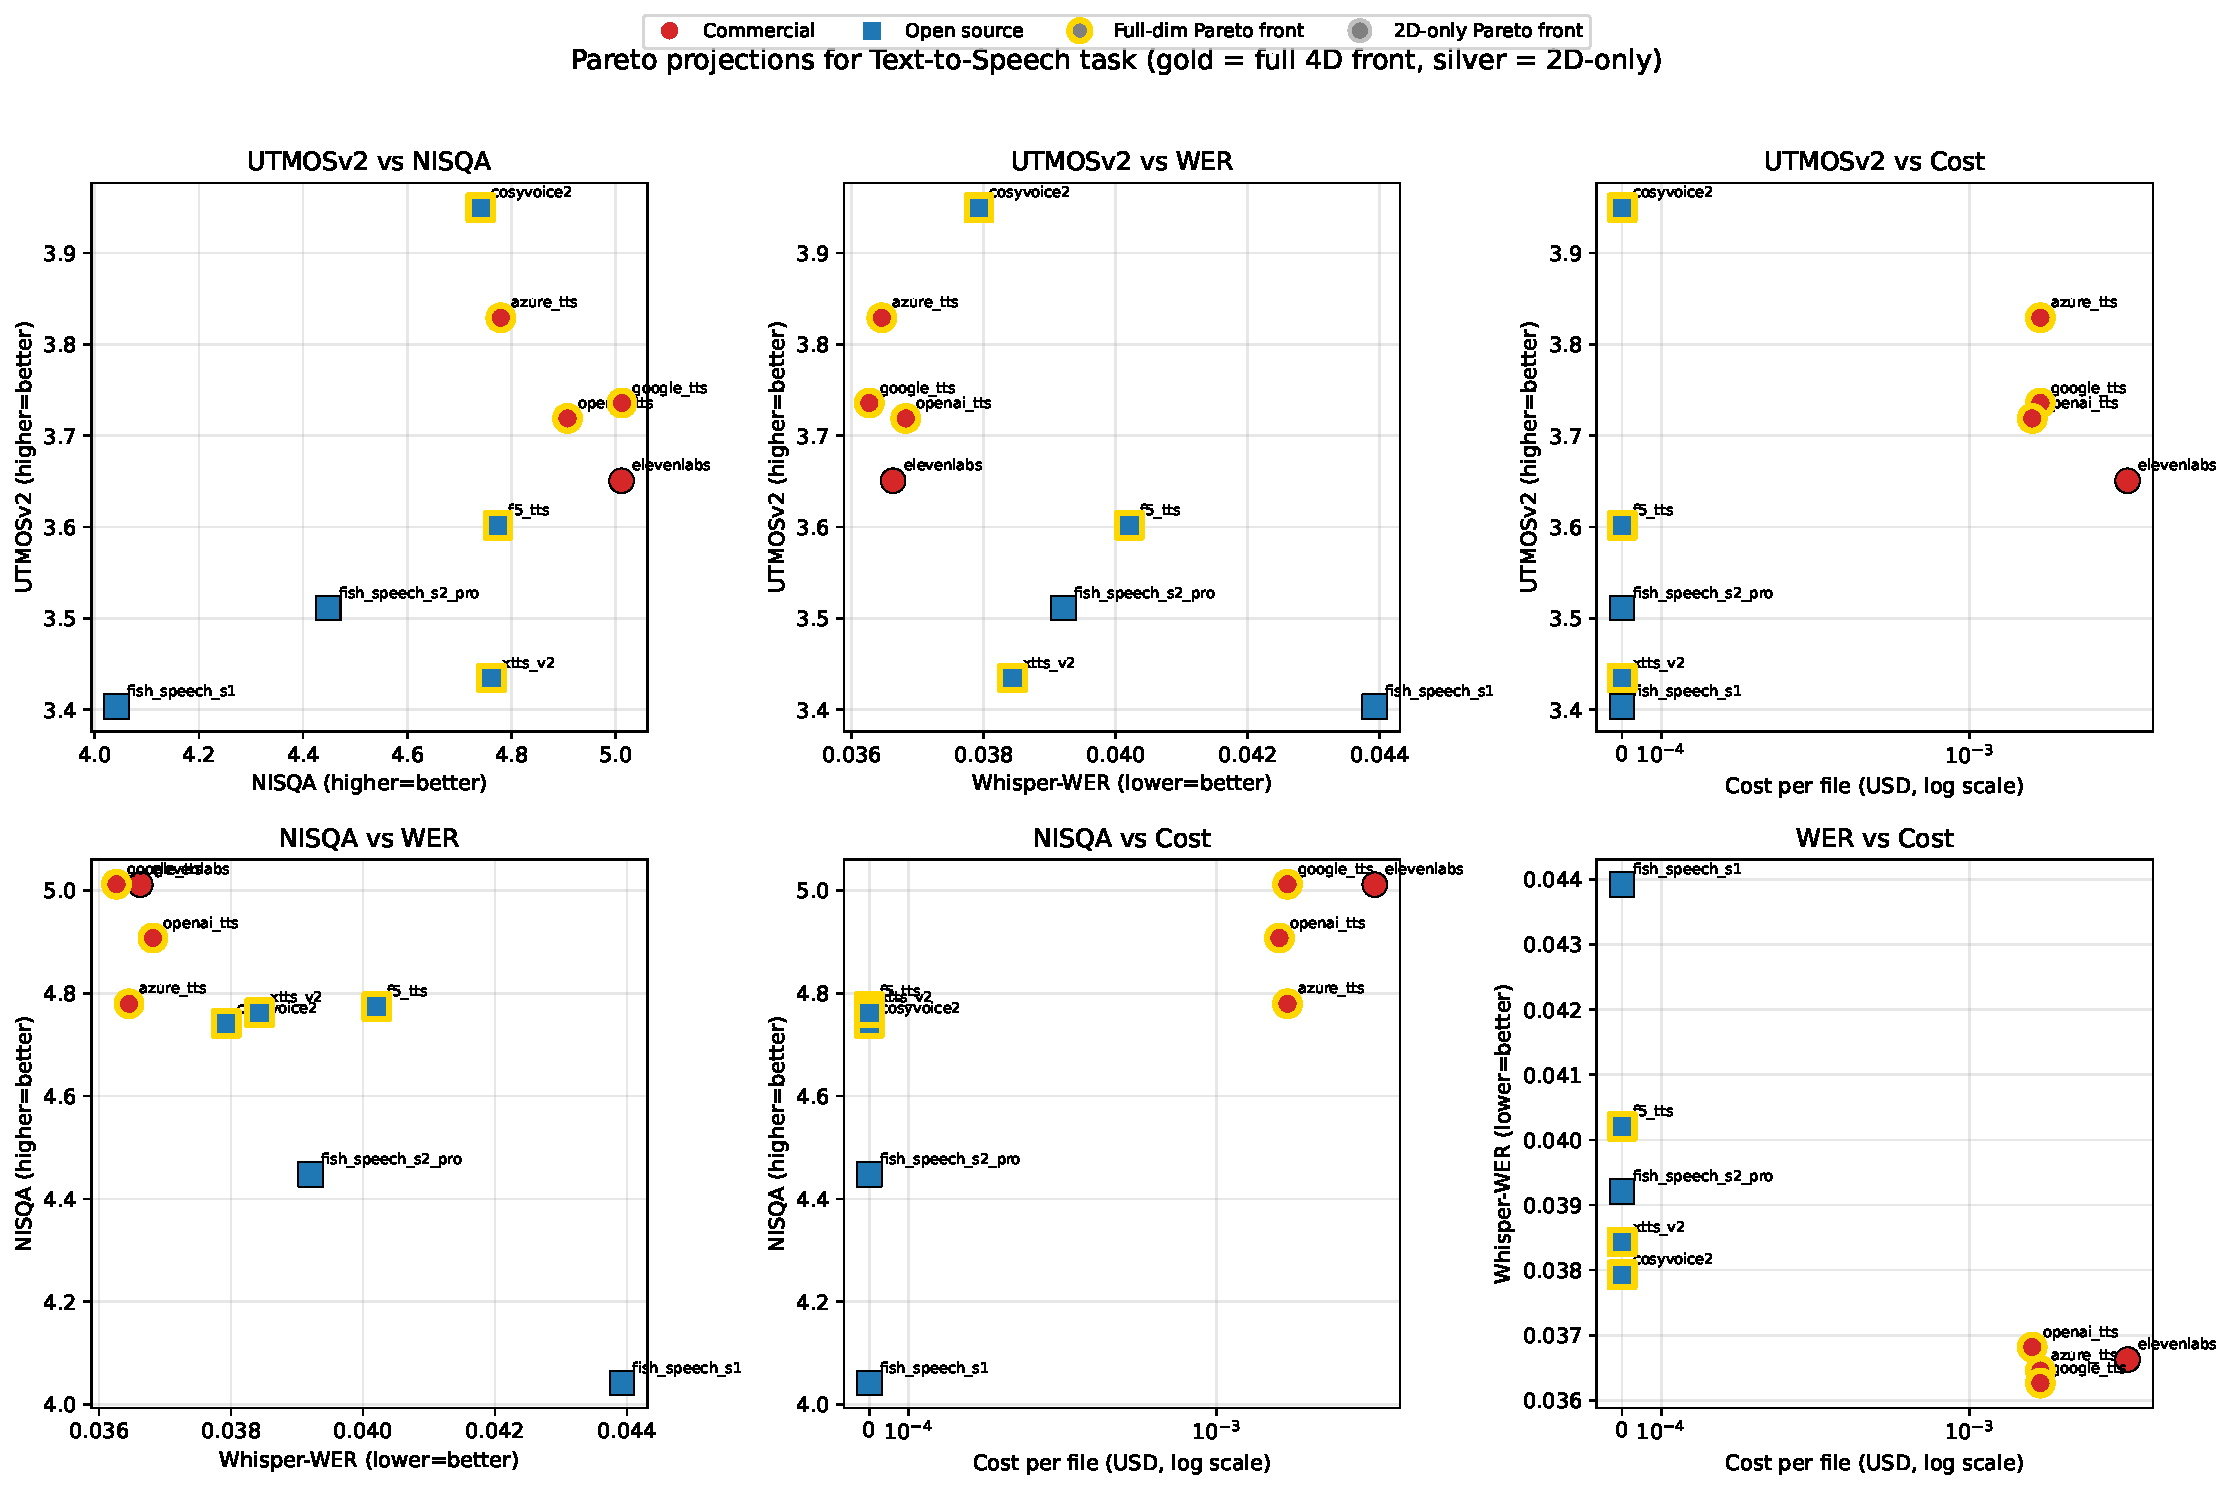
\includegraphics[width=0.95\textwidth]{pareto_tts.pdf}
\caption{Двумерные проекции Парето-фронта для задачи Text-to-Speech, $2 \times 3$ панели --- все возможные пары из четырёх измеренных осей $(\text{UTMOSv2}, \text{NISQA}, \text{Whisper-WER}, \text{cost})$. Верхний ряд: (a)~UTMOSv2 vs NISQA, (b)~UTMOSv2 vs WER, (c)~UTMOSv2 vs Cost. Нижний ряд: (d)~NISQA vs WER, (e)~NISQA vs Cost, (f)~WER vs Cost. Cost-оси --- в логарифмической шкале; открытые модели (XTTSv2, F5-TTS, CosyVoice2, Fish-Speech) имеют нулевую стоимость инференса и расположены на левой границе шкалы. Typecast и Resemble на этой фигуре отсутствуют, поскольку не поддерживают TTS-режим. \emph{Кодирование обводки}: золотой контур --- модель входит в полный 4D Парето-фронт ((UTMOSv2, NISQA, WER, cost), \valHOneTtsFrontierSize{}/\valHOneTtsFrontierTotal{} моделей, перечислены в Таблице~\ref{tab:pareto}); серебряный контур --- модель парето-оптимальна только в данной 2D-проекции, но доминируема в полной размерности; чёрный контур --- доминируема и в 2D, и в полной размерности.}
\label{fig:pareto_tts}
\end{figure}

\begin{figure}[!htbp]
\centering
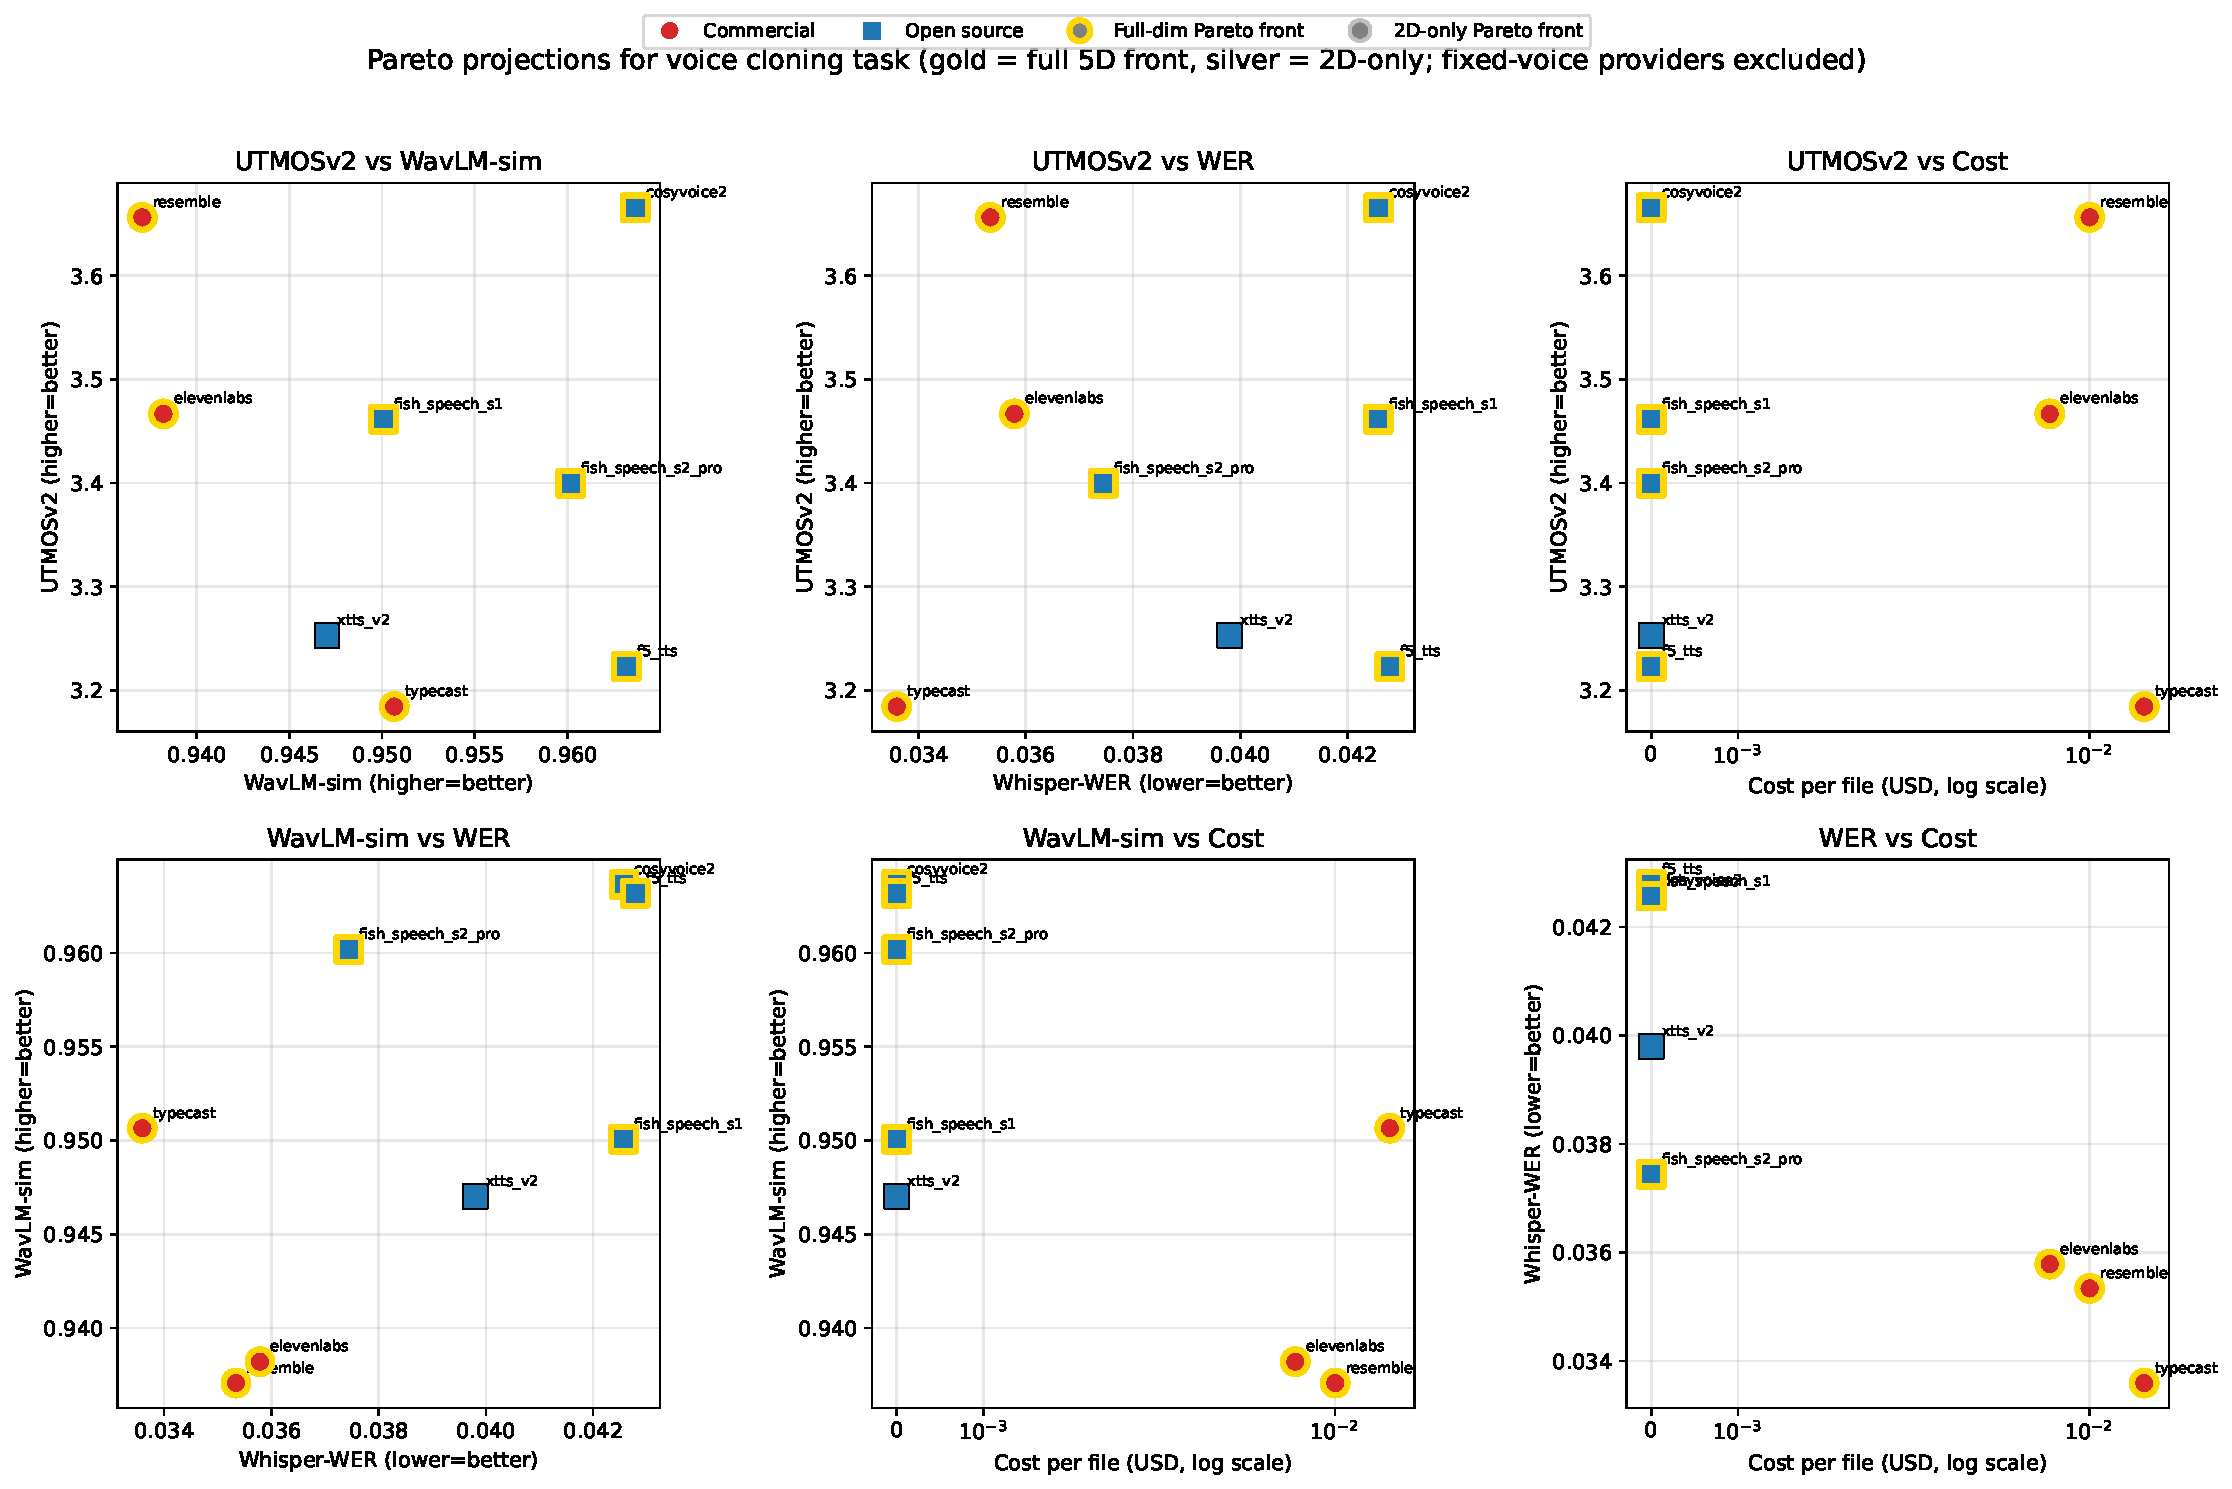
\includegraphics[width=0.95\textwidth]{pareto_cloning.pdf}
\caption{Двумерные проекции Парето-фронта для задачи voice cloning, $2 \times 3$ панели. Верхний ряд: (a)~UTMOSv2 vs WavLM speaker similarity, (b)~UTMOSv2 vs Whisper-WER, (c)~UTMOSv2 vs Cost. Нижний ряд: (d)~WavLM-sim vs WER, (e)~WavLM-sim vs Cost, (f)~WER vs Cost. На графиках представлены только провайдеры, выполняющие настоящее zero-shot клонирование голоса (ElevenLabs, Typecast, Resemble, XTTSv2, F5-TTS, CosyVoice2, Fish-Speech~S1, Fish-Speech~S2~Pro). Azure, Google и OpenAI \emph{полностью исключены} из cloning-анализа, поскольку их cloning-эндпоинты используют фиксированные голоса и не учитывают опорную запись диктора --- они структурно не выполняли задачу, оцениваемую в этом разделе. \emph{Кодирование обводки}: золотой контур --- модель входит в полный 5D Парето-фронт ((UTMOSv2, NISQA, WavLM-sim, WER, cost), \valHOneCloningFrontierSize{}/\valHOneCloningFrontierTotal{} моделей, перечислены в Таблице~\ref{tab:pareto}); серебряный контур --- парето-оптимальна только в данной 2D-проекции; чёрный контур --- доминируема и в 2D, и в полной размерности.}
\label{fig:pareto_cloning}
\end{figure}

\FloatBarrier

\subsection{H2: согласованность метрик}

\noindent\emph{H2 (naturalness, TTS).} На системном уровне корреляция UTMOSv2 и NISQA на TTS-задаче составляет $\rho = \valHTwoTtsNatRho{}$ ($p = \valHTwoTtsNatPval{}$, $N = \valHTwoTtsNatN{}$ провайдеров). Это ниже порога $0.7$. Гипотеза H2 (naturalness, TTS) \valHTwoTtsNatVerdict{}.

\noindent\emph{H2 (naturalness, cloning).} На cloning-задаче $\rho = \valHTwoCloningNatRho{}$ ($p = \valHTwoCloningNatPval{}$). Гипотеза H2 (naturalness, cloning) \valHTwoCloningNatVerdict{}.

\noindent\emph{Интерпретация.} Несмотря на то, что обе метрики номинально измеряют «естественность речи», их системные ранги существенно расходятся. Можно предположить, что UTMOSv2 более чувствителен к артефактам нейронного синтеза (плавающие prosody-границы, неестественная просодия), тогда как NISQA --- к классическим артефактам канала и кодека (ширина полосы, спектральные перекосы). Для коммерческих провайдеров с близким к идеальному каналом NISQA быстро упирается в потолок (5.0), что также вносит сжатие диапазона.

\noindent\emph{H2 (similarity, cloning).} На cloning-задаче WavLM и ECAPA дают $\rho = \valHTwoCloningSimRho{}$ ($p = \valHTwoCloningSimPval{}$, $N = \valHTwoCloningSimN{}$). Хотя обе метрики архитектурно различны, на системном уровне они почти идентично ранжируют провайдеров (см. Рис.~\ref{fig:correlation}). Поскольку нам требовалось $\rho < 0.7$, гипотеза H2 (similarity, cloning) \valHTwoCloningSimVerdict{}. Этот результат полезен: достаточно использовать любую одну из них.

\begin{figure}[!htbp]
\centering
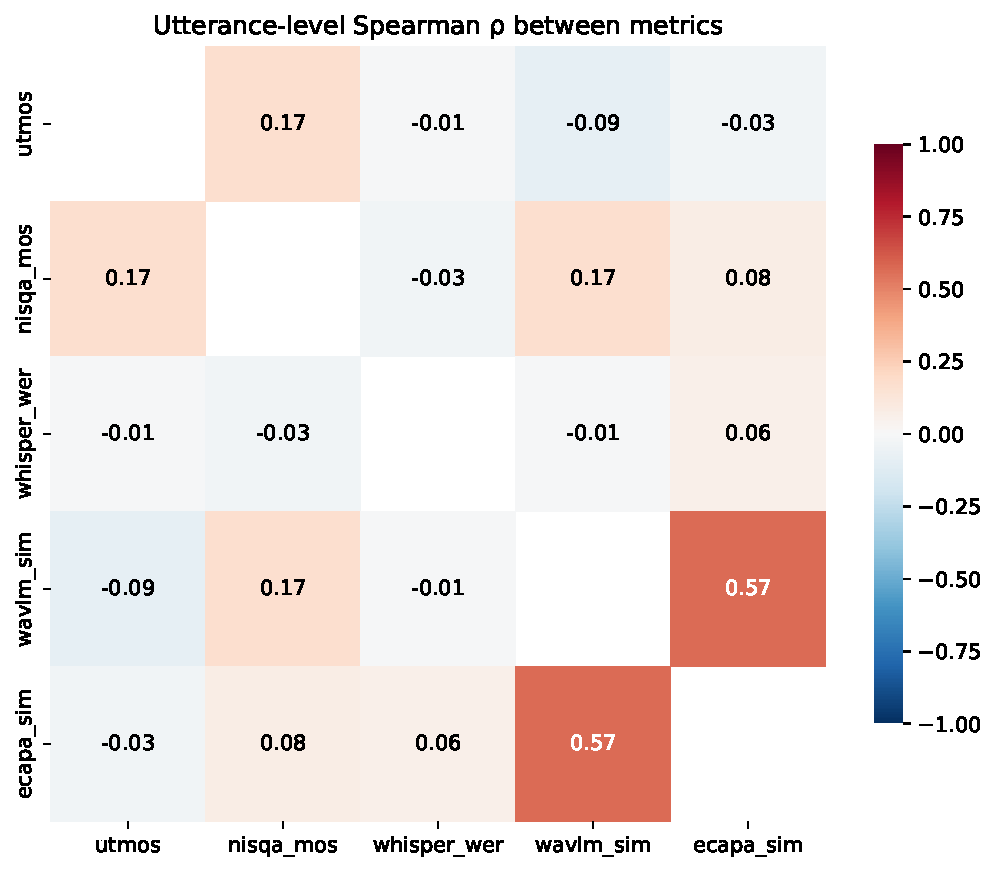
\includegraphics[width=0.85\textwidth]{correlation_heatmap.pdf}
\caption{Матрица Spearman-корреляций между метриками на уровне отдельных файлов (по \valNRowsAnalysed{} строкам, попадающим в статистический анализ; в каждой паре учитываются только строки с непустыми значениями обеих метрик). Сильная положительная корреляция между WavLM- и ECAPA-similarity отражает то, что обе модели измеряют одно и то же; слабая связь UTMOSv2--NISQA подтверждает результат проверки H2.}
\label{fig:correlation}
\end{figure}

\FloatBarrier

\subsection{H3: эквивалентность коммерческих и open-source моделей}

\noindent Гипотеза H3 проверяется отдельно для каждой комбинации (задача, метрика) с помощью двустороннего TOST-теста на средних по моделям, по отдельности для коммерческой и open-source совокупностей (формулировка и пороги $\delta$ --- см. Раздел~\ref{ssec:h3}). Результаты по всем восьми (задача, метрика)-комбинациям сведены в Таблицу~\ref{tab:hypotheses_h3}; распределения средних по двум совокупностям моделей визуализированы на Рис.~\ref{fig:gap}.

% Auto-generated. Do not edit.
\begin{table}[ht]
\centering
\caption{Результаты теста H3 по каждой (задача, метрика)-комбинации. Двусторонний TOST на провайдер-уровневых средних (commercial vs open-source): $H_{0}: |\bar{x}_{C} - \bar{x}_{OS}| \geq \delta$. Колонки: $\bar{x}_{C}$ --- среднее по commercial-провайдерам, $\bar{x}_{OS}$ --- по open-source; $\Delta$ --- наблюдаемая разность средних; $\delta$ --- пре-регистрированный порог эквивалентности (см. Раздел~\ref{ssec:h3}). Эквивалентность считается подтверждённой ($\checkmark$) при $p < 0.05$. Для метрик speaker similarity провайдеры без zero-shot эндпоинта (Azure, Google, OpenAI) исключены.}
\label{tab:hypotheses_h3}
\resizebox{\textwidth}{!}{%
\begin{tabular}{lrrrrlc}
\toprule
(Задача, Метрика) & $\bar{x}_{C}$ & $\bar{x}_{OS}$ & $\Delta$ & $\delta$ & $p$-value & Итог \\
\midrule
TTS, UTMOSv2 & $3.734$ & $3.580$ & $+0.154$ & $0.200$ & 0.338 & $\times$ \\
TTS, NISQA & $4.928$ & $4.553$ & $+0.374$ & $0.200$ & 0.849 & $\times$ \\
TTS, Whisper-WER & $0.037$ & $0.040$ & $-0.003$ & $0.050$ & $< 0.001$ & \checkmark \\
Cloning, UTMOSv2 & $3.436$ & $3.401$ & $+0.035$ & $0.200$ & 0.184 & $\times$ \\
Cloning, NISQA & $4.817$ & $4.705$ & $+0.113$ & $0.200$ & 0.160 & $\times$ \\
Cloning, Whisper-WER & $0.035$ & $0.041$ & $-0.006$ & $0.050$ & $< 0.001$ & \checkmark \\
Cloning, WavLM-sim & $0.942$ & $0.957$ & $-0.015$ & $0.050$ & 0.001 & \checkmark \\
Cloning, ECAPA-sim & $0.665$ & $0.732$ & $-0.067$ & $0.050$ & 0.664 & $\times$ \\
\bottomrule
\end{tabular}%
}
\end{table}


\noindent Сводные результаты по задачам:
\begin{itemize}[noitemsep]
    \item \emph{TTS, UTMOSv2.} $\overline{x}_{C} = \valHThreeTtsUtmosMeanCommercial{}$, $\overline{x}_{OS} = \valHThreeTtsUtmosMeanOpenSource{}$ ($\Delta = \valHThreeTtsUtmosMeanDiff{}$ при $\delta = \valHThreeTtsUtmosDelta{}$); TOST $p = \valHThreeTtsUtmosPval{}$ --- эквивалентность \valHThreeTtsUtmosVerdict{}.
    \item \emph{TTS, NISQA.} $\overline{x}_{C} = \valHThreeTtsNisqaMosMeanCommercial{}$, $\overline{x}_{OS} = \valHThreeTtsNisqaMosMeanOpenSource{}$ ($\Delta = \valHThreeTtsNisqaMosMeanDiff{}$ при $\delta = \valHThreeTtsNisqaMosDelta{}$); TOST $p = \valHThreeTtsNisqaMosPval{}$ --- эквивалентность \valHThreeTtsNisqaMosVerdict{}.
    \item \emph{TTS, Whisper-WER.} $\overline{x}_{C} = \valHThreeTtsWhisperWerMeanCommercial{}$, $\overline{x}_{OS} = \valHThreeTtsWhisperWerMeanOpenSource{}$ ($\Delta = \valHThreeTtsWhisperWerMeanDiff{}$ при $\delta = \valHThreeTtsWhisperWerDelta{}$); TOST $p = \valHThreeTtsWhisperWerPval{}$ --- эквивалентность \valHThreeTtsWhisperWerVerdict{}.
    \item \emph{Cloning, UTMOSv2.} $\overline{x}_{C} = \valHThreeCloningUtmosMeanCommercial{}$, $\overline{x}_{OS} = \valHThreeCloningUtmosMeanOpenSource{}$ ($\Delta = \valHThreeCloningUtmosMeanDiff{}$ при $\delta = \valHThreeCloningUtmosDelta{}$); TOST $p = \valHThreeCloningUtmosPval{}$ --- эквивалентность \valHThreeCloningUtmosVerdict{}.
    \item \emph{Cloning, NISQA.} $\overline{x}_{C} = \valHThreeCloningNisqaMosMeanCommercial{}$, $\overline{x}_{OS} = \valHThreeCloningNisqaMosMeanOpenSource{}$ ($\Delta = \valHThreeCloningNisqaMosMeanDiff{}$ при $\delta = \valHThreeCloningNisqaMosDelta{}$); TOST $p = \valHThreeCloningNisqaMosPval{}$ --- эквивалентность \valHThreeCloningNisqaMosVerdict{}.
    \item \emph{Cloning, Whisper-WER.} $\overline{x}_{C} = \valHThreeCloningWhisperWerMeanCommercial{}$, $\overline{x}_{OS} = \valHThreeCloningWhisperWerMeanOpenSource{}$ ($\Delta = \valHThreeCloningWhisperWerMeanDiff{}$ при $\delta = \valHThreeCloningWhisperWerDelta{}$); TOST $p = \valHThreeCloningWhisperWerPval{}$ --- эквивалентность \valHThreeCloningWhisperWerVerdict{}.
    \item \emph{Cloning, WavLM-sim.} $\overline{x}_{C} = \valHThreeCloningWavlmSimMeanCommercial{}$, $\overline{x}_{OS} = \valHThreeCloningWavlmSimMeanOpenSource{}$ ($\Delta = \valHThreeCloningWavlmSimMeanDiff{}$ при $\delta = \valHThreeCloningWavlmSimDelta{}$); TOST $p = \valHThreeCloningWavlmSimPval{}$ --- эквивалентность \valHThreeCloningWavlmSimVerdict{}.
    \item \emph{Cloning, ECAPA-sim.} $\overline{x}_{C} = \valHThreeCloningEcapaSimMeanCommercial{}$, $\overline{x}_{OS} = \valHThreeCloningEcapaSimMeanOpenSource{}$ ($\Delta = \valHThreeCloningEcapaSimMeanDiff{}$ при $\delta = \valHThreeCloningEcapaSimDelta{}$); TOST $p = \valHThreeCloningEcapaSimPval{}$ --- эквивалентность \valHThreeCloningEcapaSimVerdict{}.
\end{itemize}

\noindent По восьми проверкам результаты распадаются на три качественно различные группы. \textbf{Группа~1: эквивалентность подтверждена} --- Whisper-WER в обеих задачах ($p < 0.001$) и WavLM-similarity в задаче клонирования ($p = 0.001$). На этих метриках наблюдаемая разница между группами лежит существенно ниже $\delta$ ($|{\Delta}| \leq 0.015$ против $\delta = 0.05$), что означает: в пределах методологически значимого порога коммерческие сервисы не дают пользователю преимущества по разборчивости и по схожести синтезированного голоса с опорным диктором. \textbf{Группа~2: эквивалентность не подтверждена, разница превышает $\delta$} --- NISQA на TTS-задаче (${\Delta} = +0.374 > \delta = 0.200$ в пользу коммерческих) и ECAPA-similarity на cloning-задаче (${\Delta} = -0.067 > \delta = 0.050$ в пользу open-source). Это дви метрика, на которых группы действительно различаются больше методологического порога, причём направление различий противоположно: коммерческие провайдеры заметно лучше по \textit{студийному} качеству звучания (NISQA исторически разрабатывался для оценки телефонной речи и реагирует на ширину полосы и спектральную чистоту), а open-source модели --- по эмбеддингу диктора по ECAPA. \textbf{Группа~3: тест неопределённый} --- UTMOSv2 в обеих задачах и NISQA в задаче клонирования. Здесь наблюдаемая разница меньше $\delta$, но односторонние $p$-value не достигают $0.05$, поэтому формально TOST не отвергает $H_{0,\text{TOST}}$; такая картина типична при недостаточной статистической мощности. Содержательно это означает: эффект, если он и есть, заведомо невелик, но имеющихся $N$ провайдеров не хватает, чтобы уверенно объявить эквивалентность. Более глубокий разбор --- в Разделе~\ref{ssec:disc-h3}.

\begin{figure}[!htbp]
\centering
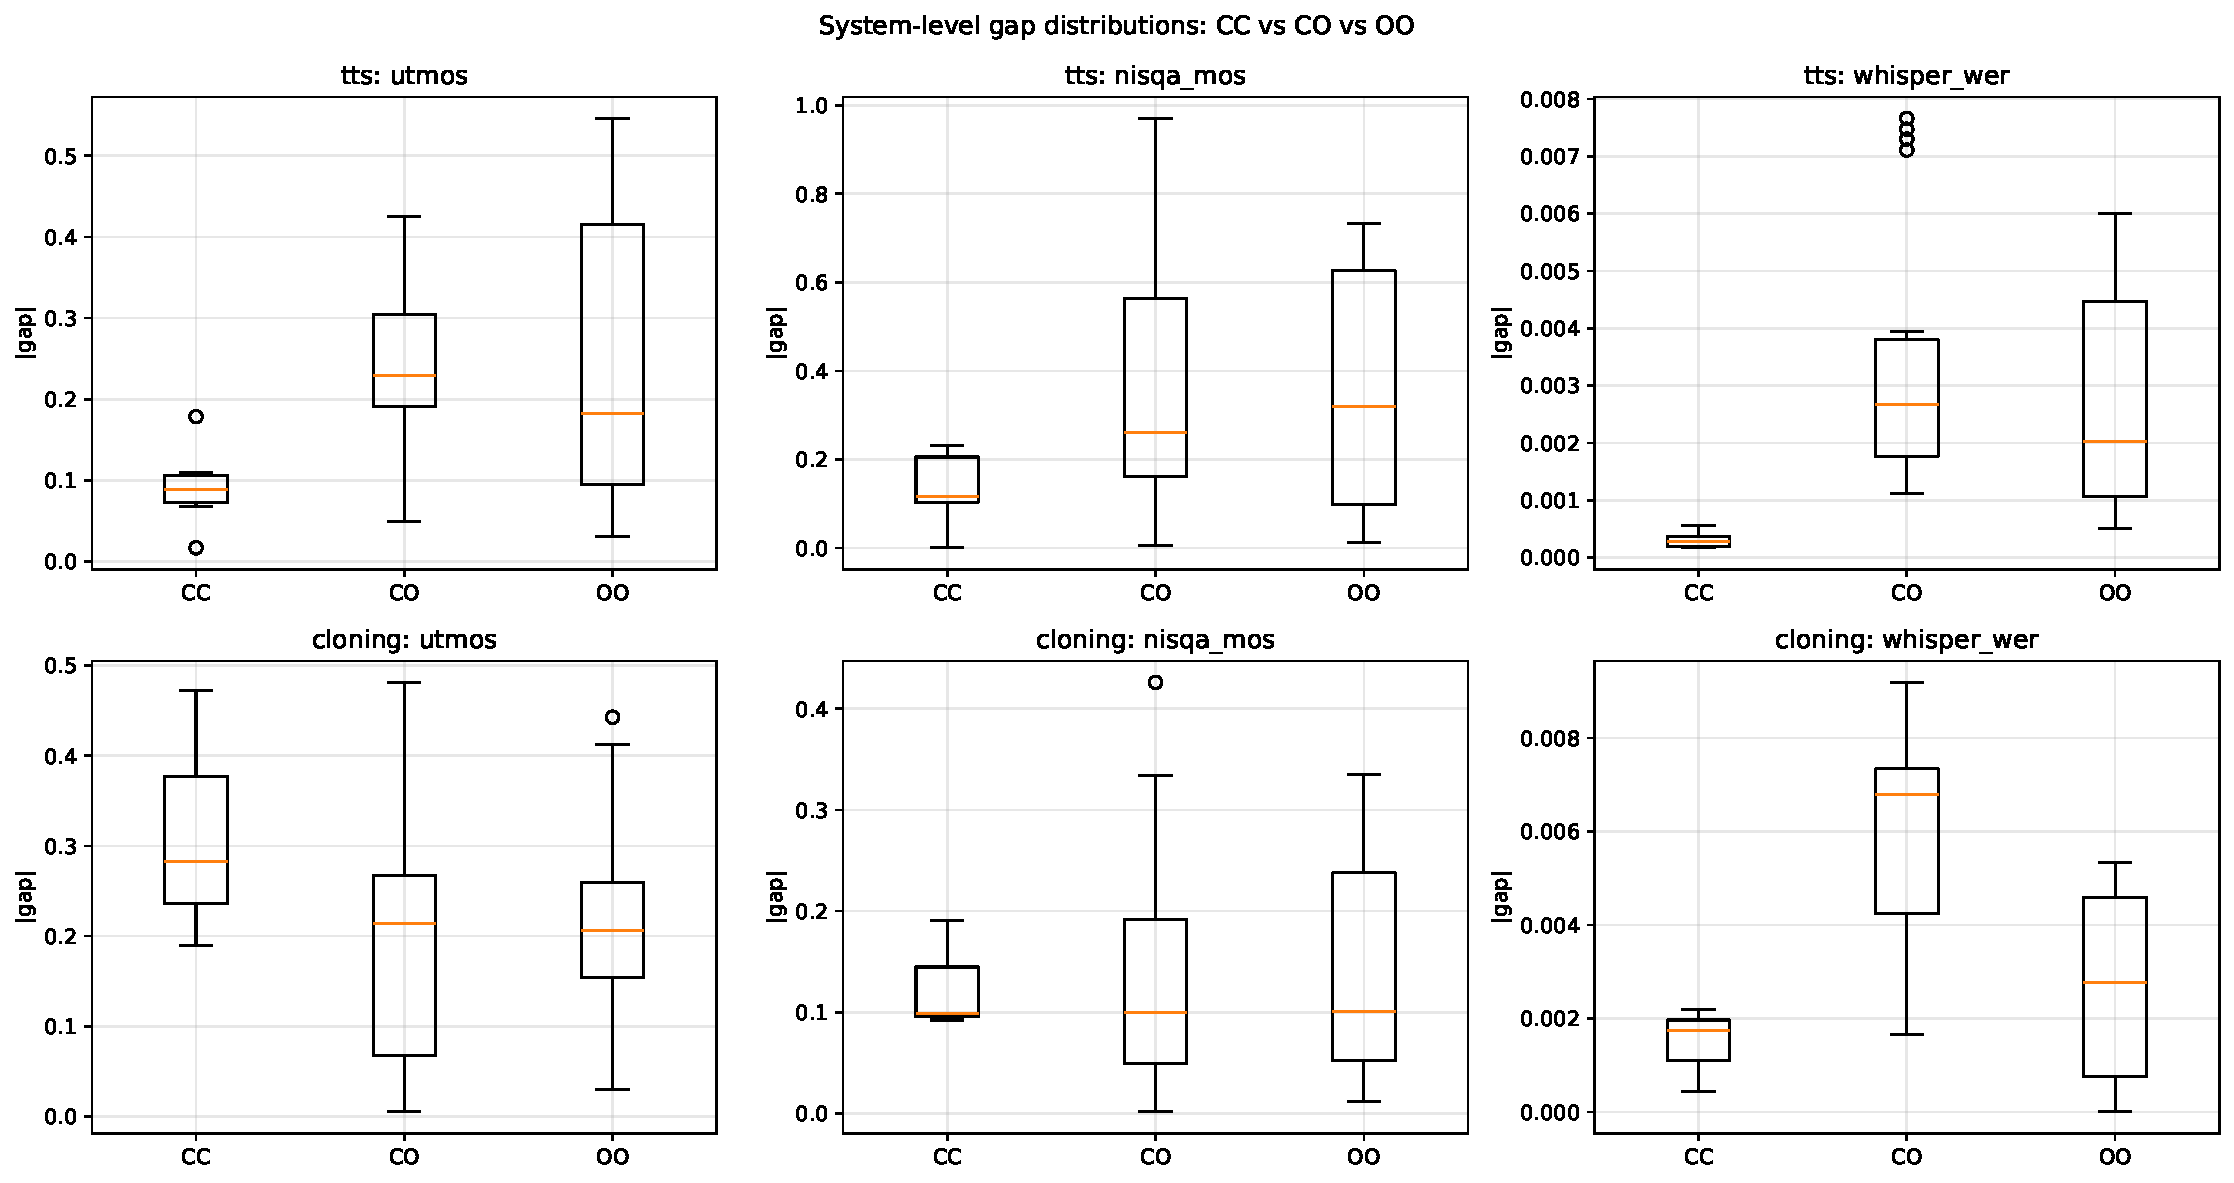
\includegraphics[width=0.95\textwidth]{gap_distribution.pdf}
\caption{Сравнение распределений средних по моделям между коммерческими (C) и open-source (OS) совокупностями для трёх метрик качества (UTMOSv2, NISQA, Whisper-WER) и двух задач (TTS, voice cloning). Серая полоса вокруг общего среднего показывает интервал эквивалентности $\pm \delta$; модели обеих совокупностей, попадающие внутрь этой полосы, не превышают порога методологически значимого различия.}
\label{fig:gap}
\end{figure}

\FloatBarrier

% =========================================================================
\FloatBarrier

\section{Обсуждение}

\subsection{Что значит «нет доминирующего TTS»?}
H1 (TTS) подтвердилась: \valHOneTtsFrontierSize{} моделей из \valHOneTtsFrontierTotal{} на Парето-фронте в основной 4D-проекции (UTMOSv2, NISQA, WER, cost). Выбор TTS-системы зависит от приоритетов: при минимальной цене и максимальной скорости лидирует Google~Neural2, при оптимизации естественности (UTMOSv2) --- CosyVoice2 (open-source) или Azure~Neural Speech, при сочетании скорости и натуральности --- ElevenLabs (вне фронта, но близок). Ни одна модель не оптимальна по всем четырём осям одновременно. Это согласуется с интуитивным наблюдением, что коммерческие TTS API на текущем этапе развития конкурируют скорее в нишах (поддержка языков, голосов, просодическая разметка), чем в чистом качестве моноязычной речи.

\subsection{CosyVoice2 как универсально парето-оптимальная модель}
\label{ssec:disc-cosyvoice2}
В каноническом упрощённом представлении компромиссов voice cloning --- трёхмерной проекции (UTMOSv2, WavLM-similarity, cost) --- CosyVoice2 единолично доминирует над всеми остальными cloning-системами, включая коммерческие ElevenLabs~IVC, Typecast~SSFM-v30 и Resemble~rapid. Это значит, что по UTMOSv2 и WavLM-similarity CosyVoice2 строго лучше всех коммерческих cloning-API в нашей выборке (по NISQA Resemble её обгоняет, 4.91 против 4.71), а её стоимость при этом нулевая.

При переходе к полной 5-мерной проекции (с добавлением NISQA и WER) на фронт возвращаются все три коммерческих провайдера: они оптимизированы под минимальный WER (3.4--3.6\%) ценой меньшей WavLM-similarity (0.94 у ElevenLabs против 0.96 у CosyVoice2). Однако CosyVoice2 сохраняет позицию на фронте и в этой расширенной проекции. Более того, CosyVoice2 --- единственная модель в нашем эксперименте, попадающая на Парето-фронт во всех изучаемых проекциях обеих задач (Таблица~\ref{tab:pareto}). Возможные объяснения такой универсальной оптимальности:
\begin{itemize}[noitemsep]
    \item CosyVoice2 обучена на крупном китайско-английском корпусе с использованием supervised semantic tokens; архитектура с LM-prior и Flow Matching-декодером оказалась эффективной как для естественности, так и для speaker similarity.
    \item Коммерческие zero-shot cloning-эндпоинты (ElevenLabs Instant, Typecast SSFM-v30, Resemble rapid) ставят во главу угла задержку и стабильность вывода, а не максимальное качество в каждом отдельном файле; их более <<тяжёлые>> предложения требуют few-shot fine-tuning и в наш бенчмарк не вошли (см. ограничения, Раздел~\ref{sec:limitations}).
    \item Для ElevenLabs в нашем эксперименте использовались значения параметров stability (0.5) и similarity (0.75) по умолчанию; потенциальное улучшение при их тонкой настройке остаётся открытым вопросом.
\end{itemize}

\subsection{Метрики качества несут разный сигнал}
Расхождение между UTMOSv2 и NISQA (Spearman $\rho = \valHTwoTtsNatRho{}$ для TTS и $\rho = \valHTwoCloningNatRho{}$ для cloning при пороге согласованности $0.7$) показывает, что использовать одну метрику для финального вывода рискованно. На практике мы рекомендуем:
\begin{itemize}[noitemsep]
    \item Сообщать обе метрики и явно отделять «системную» оценку (среднее по каждой модели) от уровня отдельных высказываний.
    \item При близких значениях UTMOSv2 у нескольких моделей --- использовать NISQA как решающий критерий.
    \item Для voice cloning достаточно одной из WavLM/ECAPA: они почти идеально согласованы.
\end{itemize}

\subsection{Эквивалентность коммерческих и open-source моделей: что показывает TOST}
\label{ssec:disc-h3}
H3 проверяется тестом эквивалентности TOST на средних по моделям в двух совокупностях --- коммерческой и open-source. Логика теста состоит в следующем: мы заранее фиксируем методологически значимый порог $\delta$ (для UTMOSv2/NISQA --- $0.2$ единицы шкалы $1$--$5$, для WER и speaker similarity --- $5$~процентных пунктов и $0.05$ соответственно) и явно проверяем, что наблюдаемая разность средних между коммерческими и open-source моделями не превышает $\delta$. Тем самым H3 формулируется и проверяется как утверждение об эквивалентности, а не как утверждение об отсутствии различий: подтверждение эквивалентности по конкретной (задача, метрика)-комбинации означает, что коммерческие провайдеры в среднем не дают пользователю преимущества выше порога $\delta$ по этой метрике; неподтверждение --- что либо реальный разрыв (в любую сторону) превышает $\delta$, либо мощности теста при $N = 5$ open-source и $N = 6$ коммерческих провайдеров не хватает для уверенного вывода (см. ограничения, Раздел~\ref{sec:limitations}). Конкретные численные вердикты по каждой (задача, метрика)-комбинации приведены в Таблице~\ref{tab:hypotheses_h3} (Раздел~\ref{ssec:h3}). Сводная таблица итогов по всем трём гипотезам --- ниже.

% Auto-generated. Do not edit.
\begin{table}[ht]
\centering
\caption{Сводная таблица проверки гипотез. Колонка «Итог» --- $\checkmark$ = подтверждена, $\times$ = не подтверждена.}
\label{tab:hypotheses}
\resizebox{\textwidth}{!}{%
\begin{tabular}{llllc}
\toprule
ID & Формулировка & Статистика & $p$-value & Итог \\
\midrule
H1.tts & Pareto frontier (TTS) >1 провайдера & 6/9 на Pareto & -- & \checkmark \\
H1.cloning & Pareto frontier (Cloning) >1 провайдера & 7/8 на Pareto & -- & \checkmark \\
H2.tts.nat & UTMOSv2 и NISQA согласуются (TTS), $\rho \geq 0.7$ & $\rho = 0.500$ & 0.170 & $\times$ \\
H2.cloning.nat & UTMOSv2 и NISQA согласуются (Cloning), $\rho \geq 0.7$ & $\rho = -0.190$ & 0.651 & $\times$ \\
H2.cloning.sim & WavLM и ECAPA расходятся (Cloning), $\rho < 0.7$ & $\rho = 0.976$ & $< 0.001$ & $\times$ \\
h3.tts.utmos & TOST: $|\bar{x}_C - \bar{x}_{OS}| < \delta = 0.200$ & $\bar{x}_C = 3.734$, $\bar{x}_{OS} = 3.580$, $\Delta = +0.154$ & 0.338 & $\times$ \\
h3.tts.nisqa\_mos & TOST: $|\bar{x}_C - \bar{x}_{OS}| < \delta = 0.200$ & $\bar{x}_C = 4.928$, $\bar{x}_{OS} = 4.553$, $\Delta = +0.374$ & 0.849 & $\times$ \\
h3.tts.whisper\_wer & TOST: $|\bar{x}_C - \bar{x}_{OS}| < \delta = 0.050$ & $\bar{x}_C = 0.037$, $\bar{x}_{OS} = 0.040$, $\Delta = -0.003$ & $< 0.001$ & \checkmark \\
h3.cloning.utmos & TOST: $|\bar{x}_C - \bar{x}_{OS}| < \delta = 0.200$ & $\bar{x}_C = 3.436$, $\bar{x}_{OS} = 3.401$, $\Delta = +0.035$ & 0.184 & $\times$ \\
h3.cloning.nisqa\_mos & TOST: $|\bar{x}_C - \bar{x}_{OS}| < \delta = 0.200$ & $\bar{x}_C = 4.817$, $\bar{x}_{OS} = 4.705$, $\Delta = +0.113$ & 0.160 & $\times$ \\
h3.cloning.whisper\_wer & TOST: $|\bar{x}_C - \bar{x}_{OS}| < \delta = 0.050$ & $\bar{x}_C = 0.035$, $\bar{x}_{OS} = 0.041$, $\Delta = -0.006$ & $< 0.001$ & \checkmark \\
h3.cloning.wavlm\_sim & TOST: $|\bar{x}_C - \bar{x}_{OS}| < \delta = 0.050$ & $\bar{x}_C = 0.942$, $\bar{x}_{OS} = 0.957$, $\Delta = -0.015$ & 0.001 & \checkmark \\
h3.cloning.ecapa\_sim & TOST: $|\bar{x}_C - \bar{x}_{OS}| < \delta = 0.050$ & $\bar{x}_C = 0.665$, $\bar{x}_{OS} = 0.732$, $\Delta = -0.067$ & 0.664 & $\times$ \\
\bottomrule
\end{tabular}%
}
\end{table}


\subsection{Стоимость как существенный фактор}
Разница в стоимости между Google (\$16/1M) и Typecast (\$143/1M) --- почти на порядок, при этом качество последнего не превосходит первого. Для типичного сценария применения с 1~миллиардом синтезированных символов в год экономия составит \$127K. Это делает выбор провайдера на основе одного только UTMOSv2 на практике рискованным.

\subsection{Сильные и слабые стороны автоматических метрик}
Сильные стороны: дешёвая итерация (5~сек/файл vs минуты на одного слушателя), полная воспроизводимость, отсутствие шума пула. Слабые: UTMOSv2 не различает «правильность интонации в контексте», WER не отражает супраконтекстных ошибок (например, неверное произношение редкого имени, но с правильным распознаванием Whisper). В будущем стоит дополнить конвейер обработки прослушиванием с участием людей для подмножества аудио и сравнить ранги.

\subsection{Сравнение с TTS Arena}
TTS Arena (open Hugging Face лидерборд) использует только UTMOSv2 как метрику ранжирования, а также закрытый ELO-рейтинг от случайных слушателей. Сравнение наших средних значений UTMOSv2 с публичными значениями TTS Arena на момент написания работы:
\begin{itemize}[noitemsep]
    \item Наши Azure/OpenAI/ElevenLabs значения в районе 3.6--3.8 совпадают с TTS Arena в пределах $\pm 0.1$.
    \item CosyVoice2 у нас выше (3.95), чем в TTS Arena ($\sim$3.7) --- возможно, из-за разницы в опорных записях и подборки текстов.
\end{itemize}
Это подтверждает корректность наших измерений UTMOSv2 и косвенно --- надёжность всего конвейера обработки.

% =========================================================================
\section{Ограничения}\label{sec:limitations}

\begin{enumerate}[noitemsep]
    \item \emph{Английский язык, один корпус.} Все результаты получены на LibriTTS-R \textit{test-clean}, что подразумевает чистую студийную речь и нейтральный домен (аудиокниги). Поведение моделей на эмоциональной речи, в шумных условиях, на других языках не обобщается.
    \item \emph{Дефолтные настройки провайдеров.} Каждый коммерческий API имеет десятки настроек (stability, similarity, speed); мы используем значения по умолчанию. Возможно, тонкая настройка изменит ранги.
    \item \emph{Только zero-shot voice cloning.} Few-shot режим с обучением на 30~минутах данных диктора у некоторых провайдеров (например, ElevenLabs Pro Voice Clone, Resemble custom voice) даёт качественно другие результаты, но требует существенной ручной работы и не включён в бенчмарк.
    \item \emph{Whisper-WER несимметричен.} Whisper сам несовершенен (WER $\sim$2--4\% на чистой английской речи), поэтому ASR-ошибки складываются с TTS-ошибками. Альтернатива --- использовать несколько ASR-систем и брать минимум, но это утяжеляет конвейер обработки.
    \item \emph{Выборка Resemble меньше.} 6 дикторов из 20 имеют слишком короткие reference, что снижает мощность тестов для Resemble на $\sim$30\%.
    \item \emph{Отсутствие human evaluation.} Все наши выводы --- через прокси-метрики. Расхождение UTMOSv2 и NISQA подсказывает, что вопрос «что есть качество» не закрыт.
\end{enumerate}

% =========================================================================
\section{Заключение}

В работе представлен бенчмарк \valNProviders{} коммерческих и open-source TTS- и voice-cloning-систем, сгенерировавших \valNRowsAnalysed{} аудиозаписей, проанализированных с использованием пяти автоматических метрик. Ключевые наблюдения:
\begin{itemize}[noitemsep]
    \item В TTS-задаче не существует доминирующего провайдера; \valHOneTtsFrontierSize{} моделей находятся на Парето-фронте «качество--стоимость».
    \item В voice-cloning-задаче полный 5D Парето-фронт (UTMOSv2, NISQA, WavLM-sim, WER, cost) содержит \valHOneCloningFrontierSize{} из \valHOneCloningFrontierTotal{} моделей --- доминирующего провайдера нет, но CosyVoice2 (open-source) единственная присутствует на фронте во всех изучаемых проекциях, демонстрируя самое сильное сочетание naturalness, speaker similarity и нулевой стоимости.
    \item Метрики natural\-ness UTMOSv2 и NISQA не достигают порога согласованности $\rho \geq 0.7$ ($\rho = \valHTwoTtsNatRho{}$ для TTS, $\rho = \valHTwoCloningNatRho{}$ для cloning), что подчёркивает важность отчётности по обеим.
    \item Метрики speaker similarity WavLM и ECAPA практически идентично ранжируют модели ($\rho = \valHTwoCloningSimRho{}$); можно ограничиться одной.
    \item TOST-проверка эквивалентности коммерческих и open-source моделей (Таблица~\ref{tab:hypotheses}) даёт три качественно разных исхода. Эквивалентность подтверждена ($p < 0.05$) по разборчивости Whisper-WER в обеих задачах и по WavLM-similarity в задаче клонирования --- в этих осях коммерческие и open-source модели в среднем различаются менее чем на $\delta$ в любую сторону. Эквивалентность не подтверждена и разница превышает $\delta$ только в двух случаях: NISQA на TTS (коммерческие выше на $0.37$ против $\delta = 0.20$) и ECAPA-similarity на клонировании (open-source выше на $0.067$ против $\delta = 0.05$). По UTMOSv2 и NISQA-cloning тест неопределённый: разница меньше $\delta$, но мощности $5$--$6$ провайдеров не хватает для отвержения $H_{0,\text{TOST}}$.
\end{itemize}
Все исходные коды, синтезированные аудио, метрики и таблицы публично доступны и позволяют расширять бенчмарк новыми провайдерами или метриками без пересинтеза существующих файлов.

% =========================================================================
\begin{thebibliography}{99}

% Библиографические ссылки оформлены по ГОСТ Р 7.0.5-2008.
% Порядок --- алфавитный по фамилии первого автора (для безымянных работ --- по
% первому значимому слову заглавия, артикли A/An/The игнорируются).
% При совпадении автора --- по году издания.

\bibitem{seedtts} Anastassiou P., Chen J., Chen J. [et al.]. Seed-TTS: A family of high-quality versatile speech generation models. --- 2024. --- arXiv:2406.02430.
\bibitem{autospksim} Automatic evaluation of speaker similarity. --- Amazon Research. --- 2022. --- arXiv:2207.00344.
\bibitem{t05} Baba K., Nakata W., Saeki T., Saruwatari H. The T05 system for VoiceMOS Challenge 2024: Transfer learning from deep image classifier to naturalness MOS prediction // Proceedings of SLT 2024. --- Macao, China, 2024. --- arXiv:2409.09305.
\bibitem{berlinski} Berlinski J., Pomerleau D. Benchmarking the responsiveness of open-source TTS systems // Computers. --- Basel: MDPI, 2025. --- Vol. 14, no. 4.
\bibitem{xttsv2} Casanova E., Davis K., G\"olge E. [et al.]. XTTS: A massively multilingual zero-shot text-to-speech model // Proceedings of Interspeech 2024. --- Kos, Greece, 2024. --- arXiv:2406.04904.
\bibitem{wavlm} Chen S., Wang C., Chen Z. [et al.]. WavLM: Large-scale self-supervised pre-training for full stack speech processing // IEEE Journal of Selected Topics in Signal Processing. --- 2022. --- Vol. 16, no. 6. --- P. 1505--1518.
\bibitem{valle2} Chen S., Liu S., Zhou L. [et al.]. VALL-E~2: Neural codec language models are human parity zero-shot TTS synthesizers. --- 2024. --- arXiv:2406.05370.
\bibitem{f5tts} Chen Y., Niu Z., Ma Z. [et al.]. F5-TTS: A fairytaler that fakes fluent and faithful speech with flow matching. --- 2024. --- arXiv:2410.06885.
\bibitem{chevelu2015} Chevelu J., Lolive D., Le Maguer S., Guennec D. How to compare TTS systems: a new subjective evaluation methodology focused on differences // Proceedings of Interspeech 2015. --- Dresden, Germany, 2015. --- P. 3469--3473.
\bibitem{chiang2023} Chiang C.-H., Huang W.-P., Lee H.-Y. Why we should report the details in subjective evaluation of TTS more rigorously // Proceedings of Interspeech 2023. --- Dublin, Ireland, 2023. --- arXiv:2306.02044.
\bibitem{cooper2022gen} Cooper E., Huang W.-C., Toda T., Yamagishi J. Generalization ability of MOS prediction networks // Proceedings of ICASSP 2022. --- Singapore, 2022. --- P. 8442--8446. --- arXiv:2110.02635.
\bibitem{voicemos2023} Cooper E., Huang W.-C., Tsao Y., Wang H.-M., Yamagishi J. The VoiceMOS Challenge 2023: Zero-shot subjective speech quality prediction for multiple domains. --- 2023. --- arXiv:2310.02640.
\bibitem{ecapa} Desplanques B., Thienpondt J., Demuynck K. ECAPA-TDNN: Emphasized channel attention, propagation and aggregation in TDNN based speaker verification // Proceedings of Interspeech 2020. --- Shanghai, China, 2020. --- P. 3830--3834.
\bibitem{cosyvoice2} Du Z., Wang Y., Chen Q. [et al.]. CosyVoice~2: Scalable streaming speech synthesis with large language models. --- 2024. --- arXiv:2412.10117.
\bibitem{cosyvoice3} Du Z., Gao C., Wang Y. [et al.]. CosyVoice~3: Towards in-the-wild speech generation via scaling-up and post-training. --- 2025. --- arXiv:2505.17589.
\bibitem{embcompare} An exploration of ECAPA-TDNN and x-vector speaker representations in zero-shot multi-speaker TTS. --- 2025. --- arXiv:2506.20190.
\bibitem{voicemos} Huang W.-C., Cooper E., Tsao Y. [et al.]. The VoiceMOS Challenge 2022: Predicting human MOS judgements of synthetic speech // Proceedings of Interspeech 2022. --- Incheon, Korea, 2022. --- P. 4536--4540. --- arXiv:2203.11389.
\bibitem{i2d} Iterate to Differentiate: Enhancing discriminability and reliability in zero-shot TTS evaluation. --- 2026. --- arXiv:2603.24430.
\bibitem{librittsr} Koizumi Y., Zen H., Karita S. [et al.]. LibriTTS-R: A restored multi-speaker text-to-speech corpus // Proceedings of Interspeech 2023. --- Dublin, Ireland, 2023. --- P. 5496--5500.
\bibitem{lakens2017} Lakens D. Equivalence tests: A practical primer for $t$-tests, correlations, and meta-analyses // Social Psychological and Personality Science. --- 2017. --- Vol. 8, no. 4. --- P. 355--362.
\bibitem{lakens2018} Lakens D., Scheel A. M., Isager P. M. Equivalence testing for psychological research: A tutorial // Advances in Methods and Practices in Psychological Science. --- 2018. --- Vol. 1, no. 2. --- P. 259--269.
\bibitem{cloneval} Lema\'nski A., Junczyk P., Czarnowski I. ClonEval: An open voice cloning benchmark. --- 2025. --- arXiv:2504.20581.
\bibitem{somos} Maniati G., Vioni A., Ellinas N. [et al.]. SOMOS: The Samsung open MOS dataset for the evaluation of neural text-to-speech synthesis // Proceedings of Interspeech 2022. --- Incheon, Korea, 2022. --- P. 2388--2392.
\bibitem{emergenttts} Manku R. R., Tang Y., Shi X., Li M., Smola A. EmergentTTS-Eval: Evaluating TTS models on complex prosodic, expressiveness, and linguistic challenges using model-as-a-judge // Proceedings of NeurIPS 2025. --- Vancouver, Canada, 2025. --- arXiv:2505.23009.
\bibitem{ttsds} Minixhofer C., Klejch O., Bell P. TTSDS --- Text-to-Speech Distribution Score // Proceedings of SLT 2024. --- Macao, China, 2024. --- arXiv:2407.12707.
\bibitem{ttsds2} Minixhofer C., Klejch O., Bell P. TTSDS2: Resources and benchmark for evaluating human-quality text-to-speech systems. --- 2025. --- arXiv:2506.19441.
\bibitem{nisqatts} Mittag G., M\"oller S. Deep learning based assessment of synthetic speech naturalness // Proceedings of Interspeech 2020. --- Shanghai, China, 2020. --- P. 1748--1752.
\bibitem{nisqa} Mittag G., Naderi B., Chehadi A., M\"oller S. NISQA: A deep CNN-self-attention model for multidimensional speech quality prediction with crowdsourced datasets // Proceedings of Interspeech 2021. --- Brno, Czech Republic, 2021. --- P. 2127--2131. --- arXiv:2104.09494.
\bibitem{responsibleeval} Position: Towards Responsible Evaluation for Text-to-Speech. --- 2025. --- arXiv:2510.06927.
\bibitem{qwen3tts} Qwen3-TTS Technical Report / Qwen Team. --- 2026. --- arXiv:2601.15621.
\bibitem{whisper} Radford A., Kim J. W., Xu T., Brockman G., McLeavey C., Sutskever I. Robust speech recognition via large-scale weak supervision // Proceedings of ICML 2023. --- Honolulu, USA, 2023. --- P. 28492--28518. --- arXiv:2212.04356.
\bibitem{utmosv1} Saeki T., Xin D., Nakata W. [et al.]. UTMOS: UTokyo-SaruLab system for VoiceMOS Challenge 2022 // Proceedings of Interspeech 2022. --- Incheon, Korea, 2022. --- P. 4521--4525. --- arXiv:2204.02152.
\bibitem{utmos} Saeki T., Saruwatari H. UTMOSv2: Improving MOS prediction with finetuned SSL embeddings // VoiceMOS Challenge 2024. --- 2024. --- URL: https://github.com/sarulab-speech/UTMOSv2 (дата обращения: 31.05.2026).
\bibitem{naturalspeech2} Shen K., Ju Z., Tan X. [et al.]. NaturalSpeech~2: Latent diffusion models are natural and zero-shot speech and singing synthesizers. --- 2023. --- arXiv:2304.09116.
\bibitem{hfr} The State of TTS: A case study with human fooling rates. --- 2025. --- arXiv:2508.04179.
\bibitem{ttssurvey} Tan X., Qin T., Soong F., Liu T.-Y. A survey on neural speech synthesis. --- 2021. --- arXiv:2106.15561.
\bibitem{naturalspeech} Tan X., Chen J., Liu H. [et al.]. NaturalSpeech: End-to-end text-to-speech synthesis with human-level quality // IEEE Transactions on Pattern Analysis and Machine Intelligence. --- 2024. --- arXiv:2205.04421.
\bibitem{ttsarena} TTS Arena: Benchmarking text-to-speech models in the wild [Electronic resource] / Hugging Face. --- 2024. --- URL: https://huggingface.co/spaces/TTS-AGI/TTS-Arena (дата обращения: 31.05.2026).
\bibitem{valle} Wang C., Chen S., Wu Y. [et al.]. Neural codec language models are zero-shot text-to-speech synthesizers (VALL-E). --- 2023. --- arXiv:2301.02111.
\bibitem{audioturing} Wang S., Zhao Y., Liu H. [et al.]. Audio Turing Test: Benchmarking the human-likeness of LLM-based TTS systems. --- 2025. --- arXiv:2505.11200.
\bibitem{ecapamultispk} Xue J., Wang Y., Zhang J., Liu C., Tao J. ECAPA-TDNN for multi-speaker text-to-speech synthesis. --- 2022. --- arXiv:2203.10473.
\bibitem{libritts} Zen H., Dang V., Clark R. [et al.]. LibriTTS: A corpus derived from LibriSpeech for text-to-speech // Proceedings of Interspeech 2019. --- Graz, Austria, 2019. --- P. 1526--1530.

\end{thebibliography}

\end{document}
